\documentclass[11pt,a4paper]{article}
\usepackage[margin=2cm]{geometry}
\usepackage{amsmath,amssymb}
\usepackage{tcolorbox}
\usepackage{booktabs}
\usepackage{enumitem}
\usepackage{hyperref}
\usepackage{xcolor}
\usepackage{fancyhdr}
\usepackage{tikz}
\usepackage{listings}

\tcbuselibrary{breakable,skins}

% ── Listings config (monospace that wraps inside boxes) ─────────────────────
\lstset{
  basicstyle=\ttfamily\small,
  breaklines=true,
  breakatwhitespace=false,
  breakautoindent=true,
  postbreak=\mbox{\textcolor{gray}{$\hookrightarrow$}\space},
  columns=fullflexible,
  keepspaces=true,
  xleftmargin=0pt,
  xrightmargin=0pt,
  aboveskip=4pt,
  belowskip=4pt,
  frame=none,
  commentstyle=\color{gray},
}

% ── Box definitions (all use enhanced jigsaw to never clip content) ─────────
\newtcolorbox{definitionbox}[1]{colback=blue!5, colframe=blue!60!black,
  fonttitle=\bfseries, title=#1, breakable, enhanced jigsaw}

\newtcolorbox{conceptbox}[1]{colback=red!5, colframe=red!60!black,
  fonttitle=\bfseries, title=#1, breakable, enhanced jigsaw}

\newtcolorbox{examplebox}[1]{colback=green!5, colframe=green!50!black,
  fonttitle=\bfseries, title=#1, breakable, enhanced jigsaw}

\newtcolorbox{notebox}[1]{colback=orange!5, colframe=orange!60!black,
  fonttitle=\bfseries, title=#1, breakable, enhanced jigsaw}

\newcommand{\kemark}{\textcolor{red!70!black}{\textbf{[EXAM-RELEVANT]}}}
\newcommand{\kbg}{\textcolor{gray}{\textbf{[BACKGROUND]}}}
\newcommand{\kt}[1]{\par\vspace{0.3em}\colorbox{yellow!60}{\parbox{\dimexpr\linewidth-2\fboxsep}{#1}}\vspace{0.3em}}

\pagestyle{fancy}
\fancyhf{}
\lhead{AC Lecture 1 --- Cheatsheet}
\rhead{Jawad M.K. Qayyum}
\rfoot{\thepage}

\setlength{\parindent}{0pt}
\setlength{\parskip}{0.4em}

\begin{document}

\begin{center}
{\Huge\bfseries AC Lecture 1}\\[0.5em]
{\LARGE Intro + Turing Machines}\\[0.3em]
{\large The Complete Guide to ``What is a Problem?'' and ``What is an Algorithm?''}\\[1em]
{\normalsize Algorithms and Computability --- Semester 6}\\
{\normalsize Cheatsheet for split-view study with slides}
\end{center}

\vspace{1em}
\tableofcontents
\newpage

%═══════════════════════════════════════════════════════════════════════════════
\section{The Big Picture --- Why This Course Exists}
%═══════════════════════════════════════════════════════════════════════════════

\begin{conceptbox}{Before We Start --- Why Should You Care About This Course?}
Imagine you're a software developer and your boss asks: ``Write me a program that checks whether any given program will crash.'' You spend weeks, months --- and you can't do it. Is it because you're bad at programming? \textbf{No.} It's because it's \textbf{mathematically impossible}. No one can do it. Not now, not ever.

But how do you \textit{prove} something is impossible? You can't just say ``I tried really hard and failed.'' You need a \textbf{formal definition} of what a ``program'' and a ``problem'' even \textit{are}. That's what this course gives you.

\textbf{Three things you'll learn:}
\begin{enumerate}[nosep]
\item Some problems are \textbf{impossible} to solve (not hard --- literally impossible)
\item Some problems are \textbf{possible but impractical} (would take longer than the age of the universe)
\item There are clever tricks to \textbf{cope} with hard problems anyway
\end{enumerate}

The lecture opens with three stories that set up each of these themes.
\end{conceptbox}

The slides open with three stories. Each one sets up a different theme of the course. These are \kbg{} for the exam but they are the \textit{motivation} for every definition that follows.

%───────────────────────────────────────────────────────────────────────────────
\subsection{Story 1: An Algorithm --- Primality Testing (slides 1--2)}

\begin{conceptbox}{Input Size vs.\ Input Value --- The Trap}

\textbf{Analogy:} Imagine you order a package online. The \textbf{weight} of the package is 50 kg. But the \textbf{shipping label} that describes the package is just a small piece of paper saying ``50 kg.'' The delivery truck's effort depends on the \textit{weight} (50 kg), but the label's \textit{length} is just 4 characters. If the package weighs 50,000 kg, the label says ``50000 kg'' --- only 8 characters, but the effort is 1000x harder. \textbf{The label is short but the work is huge.} Same with algorithms: the input \textit{string} is short ($\log n$ digits), but the \textit{work} can be enormous ($\sqrt{n}$ steps).

\textbf{The problem:} Given a number $n$, is it prime?

\textbf{The naive algorithm:} This algorithm checks whether $n$ is prime by trying every possible divisor from 2 up to $\sqrt{n}$. If any of them divides $n$ evenly, $n$ is not prime. If none of them do, $n$ is prime. The key idea: if $n$ has a factor bigger than $\sqrt{n}$, it must also have one smaller than $\sqrt{n}$, so checking up to $\sqrt{n}$ is enough.

\begin{lstlisting}
    def is_prime(n):                              # Input: the number to test
        for i in range(2, floor(sqrt(n)) + 1):    # Try each divisor from 2 to sqrt(n)
            if n % i == 0:                         # If i divides n with no remainder
                return False                       # n is NOT prime (found a divisor)
        return True                                # No divisor found -- n IS prime
\end{lstlisting}

This checks $\lfloor\sqrt{n}\rfloor - 1$ divisors. That's $O(\sqrt{n})$ iterations. Sounds fast, right?

\textbf{The trap --- let's do the actual math:}

Say $n = 1{,}000{,}000{,}000$ (one billion). Then:
\begin{itemize}[nosep]
\item $\sqrt{n} = 31{,}623$ iterations. Seems manageable.
\item But wait: \textbf{what is the input size?} The input is the \textit{string} ``1000000000''. That's \textbf{10 characters} long.
\item In binary, $n$ needs $k = \lfloor\log_2 n\rfloor + 1$ bits. For $n = 10^9$, that's about $k = 30$ bits.
\item So the input has size $k = 30$, but the algorithm does $\sqrt{n} = \sqrt{2^k} = 2^{k/2}$ iterations.
\end{itemize}

\textbf{$2^{k/2}$ is \textbf{exponential} in $k$.} The algorithm looks at the \textit{value} of $n$ and says $O(\sqrt{n})$, but computer science measures complexity in the \textit{size of the input representation}. In terms of input size $k$:

$$O(\sqrt{n}) = O(\sqrt{2^k}) = O(2^{k/2})$$

That's \textbf{exponential}, not polynomial. For $k = 100$ bits ($n \approx 10^{30}$), the algorithm needs $2^{50} \approx 10^{15}$ iterations. That takes years.

\textbf{The real solution:} In 2002, Agrawal, Kayal, and Saxena found an algorithm (AKS) that runs in time $O(k^c)$ for some constant $c$ --- that's \textbf{polynomial in input size}. They won the G\"odel Prize and Fulkerson Prize for this.

\kt{``Efficient'' in this course means polynomial in the \textbf{number of symbols in the input} (i.e., $k = |\text{string}|$), NOT in the numeric value. $O(\sqrt{n})$ is exponential because $n = 2^k$.}
\end{conceptbox}

\textbf{Why this matters for AC:} When we study complexity classes P and NP (Lectures 5--7), ``polynomial time'' always means polynomial in the \textit{length of the input string}. If you confuse input size with input value, every complexity argument will seem wrong to you.

%───────────────────────────────────────────────────────────────────────────────
\subsection{Story 2: A Thief --- The Knapsack Problem (slide 3)}

\begin{examplebox}{Greedy $\neq$ Optimal}

\textbf{Analogy:} You're at a buffet with a small plate. You want maximum deliciousness. The greedy strategy: always grab the tastiest-looking dish first. But what if the tastiest dish is a huge steak that takes up your whole plate, and you miss out on three amazing small dishes that together would be way better? \textbf{Greedy (``always pick the best-looking option right now'') doesn't always give the best overall result.} Some problems require you to think ahead --- and that thinking-ahead can be astronomically expensive.

\textbf{Setup:} A thief has a knapsack that holds 15 kg. Available items:

\begin{center}
\begin{tabular}{lccc}
\toprule
\textbf{Item} & \textbf{Weight} & \textbf{Value} & \textbf{Value/kg} \\
\midrule
Item 1 & 12 kg & \$100 & \$8.33/kg \\
Item 2 & 5 kg & \$60 & \$12.00/kg \\
Item 3 & 7 kg & \$160 & \$22.86/kg \\
\bottomrule
\end{tabular}
\end{center}

\textbf{Greedy approach} (pick highest value/kg first):
\begin{enumerate}[nosep]
\item Take item 3 (7 kg, \$160). Remaining capacity: 8 kg.
\item Take item 2 (5 kg, \$60). Remaining capacity: 3 kg.
\item Item 1 doesn't fit. \textbf{Total: \$220, weight 12 kg.}
\end{enumerate}

Wait --- actually in the slides the greedy picks items 1+2 = \$160 and the optimal is items 2+3 = \$220. Let me re-examine. The slides say greedy gives \$160, optimal gives \$220. The exact numbers depend on the slide's specific instance, but the point is:

\kt{Greedy algorithms don't always find the optimal solution. Some problems are fundamentally \textbf{hard} --- there might be no efficient algorithm. This is what NP-hardness means (Lectures 6--7).}
\end{examplebox}

%───────────────────────────────────────────────────────────────────────────────
\subsection{Story 3: Collatz --- The Unsolvable (slide 4)}

\begin{conceptbox}{Some Problems Cannot Be Solved At All}

\textbf{Analogy:} Imagine a maze where the paths keep changing as you walk. You enter, take a left, take a right, and suddenly the maze rearranges itself. Will you ever find the exit? Maybe, maybe not. Now imagine someone asks you: ``Given ANY maze blueprint, can you tell me in advance whether the person will ever get out?'' For some mazes, yes. But can you build a \textbf{universal} maze-analyzer that works for ALL possible mazes? \textbf{No.} Some questions about future behavior are fundamentally unanswerable. That's what ``uncomputability'' means --- not ``we haven't figured it out yet'' but ``it's mathematically proven to be impossible.''

\textbf{The Collatz function:} This function takes a positive integer $n$ and repeatedly applies a simple rule: if $n$ is even, halve it; if odd, triple it and add 1. It keeps going until it reaches 1. The conjecture is that it ALWAYS reaches 1 eventually, no matter what $n$ you start with --- but nobody has been able to prove it.

\begin{lstlisting}
    def collatz(n):                         # Input: a positive integer
        if n == 1:                          # Base case: we reached 1
            return True                     # Done -- the sequence terminated
        if n % 2 == 0:                      # If n is even
            return collatz(n // 2)          # Halve it and recurse
        else:                               # If n is odd
            return collatz(3 * n + 1)       # Triple it, add 1, and recurse
\end{lstlisting}

\textbf{Does \texttt{collatz(n)} return \texttt{True} for every positive integer $n$?}

Nobody knows. It's been checked for all $n \leq 2^{68}$ (that's $\approx 3 \times 10^{20}$), and the answer is always True. But that's not a proof.

\textbf{Let's trace a few values to see the function in action:}
\begin{itemize}[nosep]
\item $\texttt{collatz}(6)$: $6 \to 3 \to 10 \to 5 \to 16 \to 8 \to 4 \to 2 \to 1$. True.
\item $\texttt{collatz}(7)$: $7 \to 22 \to 11 \to 34 \to 17 \to 52 \to 26 \to 13 \to 40 \to 20 \to 10 \to 5 \to \ldots \to 1$. True.
\item $\texttt{collatz}(27)$: takes 111 steps, reaches a peak of 9232 before eventually hitting 1.
\end{itemize}

\textbf{Now the deeper question the slide asks:} Can you write a program that, given \textit{any} function like \texttt{collatz}, determines whether it always returns True?

The answer is \textbf{provably NO}. This is essentially the Halting Problem (Lecture 2). There exist problems that \textbf{no algorithm can solve} --- not because we haven't found the right algorithm, but because it's \textit{mathematically impossible}.

\kt{This course has three layers: (1) What CAN be computed? (Lectures 1--4: computability), (2) What can be computed EFFICIENTLY? (Lectures 5--7: P vs NP), (3) How to cope with hard problems? (Lectures 8--13: algorithms).}
\end{conceptbox}

%───────────────────────────────────────────────────────────────────────────────
\subsection{Course Overview --- The Three-Part Structure (slides 5--6)}

\textbf{Slide 5 says:} In previous courses you've seen specific algorithms (sorting, graph search) and analyzed their runtime. This course asks the \textit{meta-questions}:

\begin{enumerate}[nosep]
\item Can every problem be solved (efficiently) by an algorithm?
\item Actually, what IS an algorithm? And what IS a problem?
\item How can we still solve \textit{hard} problems?
\end{enumerate}

\textbf{The three parts:}

\begin{center}
\renewcommand{\arraystretch}{1.4}
\begin{tabular}{llp{8cm}}
\toprule
\textbf{Part} & \textbf{Lectures} & \textbf{Topic} \\
\midrule
1 --- Computability & L1--L5 & What can be computed at all? Turing machines, Church-Turing thesis, undecidability, reductions. \textit{Some problems have NO solution.} \\
2 --- Complexity & L6--L9 & What can be computed \textit{efficiently}? P, NP, NP-completeness, SAT. \textit{Some problems have solutions but (probably) no fast ones.} \\
3 --- Coping & L10--L13 & How to solve hard problems anyway. Backtracking, branch-and-bound, LP, ILP, approximation, amortized analysis, DP. \\
\bottomrule
\end{tabular}
\end{center}

\textbf{Lecture 1 is the foundation of Part 1.} Today we define what a ``problem'' is (= language) and what an ``algorithm'' is (= Turing machine). Everything else builds on these two definitions.


%───────────────────────────────────────────────────────────────────────────────
\subsection{Course Formalities (slides 7--9)}

\begin{itemize}[nosep]
\item \textbf{Literature:} CLRS (Introduction to Algorithms, 3rd/4th ed --- same book as Semester 2) + Hubie Chen: \textit{Computability and Complexity} (MIT Press, ISBN 9780262048620)
\item \textbf{Schedule:} Lectures Thu 12:30--14:15 + Fri 8:15--10:00. Exercises Thu 14:30--16:15 + Fri 10:15--11:45.
\item \textbf{Exercises} roughly every other week. \textbf{Essential preparation for the exam.}
\item \textbf{Workload:} ~150 hours. Lectures + exercises = only 1/3. The rest is reading, revising, exam prep.
\item \textbf{Exam:} Main exam written, re-exam (tentatively) oral.
\item \textbf{Contact:} mzi@cs.aau.dk. Questions: (1) discuss in group, (2) Moodle forum, (3) email.
\end{itemize}


%═══════════════════════════════════════════════════════════════════════════════
\newpage
\section{Setting the Stage: Problems = Languages (slides 10--17)}
%═══════════════════════════════════════════════════════════════════════════════

\begin{conceptbox}{Intuition: Why Do We Need to Define ``Problem'' Formally?}
You already know what a ``problem'' is in everyday life: ``Is 17 prime?'', ``Can I drive from Aalborg to Copenhagen in 4 hours?'' But in computer science, we need to be \textbf{extremely precise} because we want to prove things like ``this problem is impossible to solve.''

\textbf{Analogy:} Imagine you run a restaurant. A ``menu item'' is an everyday concept --- everyone knows what it is. But if you want to write software to manage your menu, you need a precise data structure: name (string), price (float), category (enum). The informal concept becomes a formal object.

Same thing here: an informal ``problem'' becomes a formal ``language'' (a set of strings). This isn't because mathematicians love complexity --- it's because \textbf{you can't prove impossibility without precision}.

\textbf{The key trick:} We encode EVERYTHING (numbers, graphs, programs) as strings of symbols. Then every problem becomes: ``Is this string in this set?'' One framework to rule them all.
\end{conceptbox}

\subsection{The Motivating Question (slide 11)}

The slide just says: \textit{``Actually, what is an algorithm? And what is a problem?''}

This is the question the entire lecture answers:
\begin{itemize}[nosep]
\item A \textbf{problem} = a \textbf{formal language} (Section 2)
\item An \textbf{algorithm} = a \textbf{Turing machine} (Section 3)
\end{itemize}

%───────────────────────────────────────────────────────────────────────────────
\subsection{What is a Problem? --- Decision Problems (slide 12)}

\begin{definitionbox}{Decision Problem}
\textbf{Analogy:} Think of a bouncer at a club. The bouncer has ONE job: look at each person in line and say ``yes, you're in'' or ``no, you're not.'' That's a decision problem --- a yes/no question applied to many different inputs (people). The bouncer doesn't say ``you're 73\% allowed in'' --- it's strictly binary. In formal world: bouncer = algorithm, person = input, club rules = the problem definition.

\textbf{Plain English:} A decision problem is a \textbf{yes/no question} that you can ask about many different inputs. Not ``what's the shortest path?'' but ``is there a path shorter than 10?''

\textbf{Examples from the slide:}
\begin{enumerate}[nosep]
\item Is a given number prime?
\item Does a given graph have a path from source to destination?
\item Can the thief fit \$250 of loot in his knapsack?
\item Is a given formula of propositional logic satisfiable?
\item Can a graph be colored with 3 colors so no neighbors share a color?
\item Does a given program ever output \texttt{False}?
\end{enumerate}

\textbf{General format:} A yes/no question over a (typically infinite) set of inputs.
\end{definitionbox}

%───────────────────────────────────────────────────────────────────────────────
\subsection{The Abstraction: Everything is a String (slide 13)}

\begin{conceptbox}{Why We Encode Everything as Strings}
\textbf{The problem:} Inputs come in all types --- numbers, graphs, formulas, programs, sets of inequalities, polynomials. We can't build a separate theory for each type.

\textbf{The solution:} Encode everything as a \textbf{sequence of symbols} (a string/word):
\begin{itemize}[nosep]
\item A \textbf{number} is encoded in binary or decimal: $17 \to$ ``17'' or ``10001''
\item A \textbf{graph} is encoded by (a linearization of) its adjacency matrix: $\begin{pmatrix} 0 & 1 \\ 1 & 0 \end{pmatrix} \to$ ``0110''
\item A \textbf{program} is given by its source code: the Python file IS already a string
\end{itemize}

Once everything is a string, we have one unified framework. A ``problem'' becomes: given a string, does it belong to a certain set of strings?
\end{conceptbox}

%───────────────────────────────────────────────────────────────────────────────
\subsection{Formal Languages --- Complete Refresher (slide 14)}

\begin{notebox}{Intuition: What Are Formal Languages and Why Do You Need Them?}
Think of formal languages as a very precise way of describing ``collections of texts.'' You already use this idea every day:
\begin{itemize}[nosep]
\item All valid Danish CPR numbers = a language (10-digit strings with specific rules)
\item All valid email addresses = a language (strings matching a pattern like \texttt{name@domain.com})
\item All prime numbers written in decimal = a language (\texttt{``2''}, \texttt{``3''}, \texttt{``5''}, \texttt{``7''}, \texttt{``11''}, ...)
\item All syntactically correct Python programs = a language
\end{itemize}

To define a language precisely, you need three things:
\begin{enumerate}[nosep]
\item \textbf{An alphabet} --- what symbols are you allowed to use? (Like: digits 0-9, or letters a-z, or binary 0/1)
\item \textbf{Words} --- sequences of those symbols (like ``hello'' or ``10110'' or ``17'')
\item \textbf{The language itself} --- which words are ``in'' and which are ``out'' (like: ``17'' is in the prime language, ``15'' is out)
\end{enumerate}

The next definitions formalize each of these three ingredients. You saw them in Semester 1 --- here's a refresher with more intuition.
\end{notebox}

This is all from Semester 1 (Theoretical Foundations). You scored 4 there, so let's be thorough.

\begin{definitionbox}{Alphabet ($\Sigma$) \kemark}
\textbf{Analogy:} A Scrabble bag. It contains a fixed set of tiles (A-Z). You can only make words using tiles from the bag. If the bag only has tiles \{0, 1\}, you can only make binary words. The bag = the alphabet.

\textbf{Plain English:} An alphabet is a finite set of symbols --- the ``letters'' you're allowed to use. Think of it as the keys on a restricted keyboard.

\textbf{Formal:} An \textbf{alphabet} is a finite, nonempty set of letters.

\textbf{Breaking Down the Notation:}
\begin{itemize}[nosep]
\item We always use $\Sigma$ (capital sigma) for the alphabet
\item ``Finite'' means it has a fixed number of symbols (could be 2, could be 100, but not infinite)
\item ``Nonempty'' means it has at least one symbol
\end{itemize}

\textbf{Examples from the slide:}
\begin{itemize}[nosep]
\item $\mathbb{B} = \{0, 1\}$ --- the binary alphabet. Two symbols.
\item $\{0, 1, 2, 3, 4, 5, 6, 7, 8, 9\}$ --- decimal digits. Ten symbols.
\item $\{a, b, c, \ldots, z\}$ --- the roman alphabet. Twenty-six symbols.
\item $\Sigma_L = \{\neg, \land, \lor, (, ), p, 0, 1, 2, 3, 4, 5, 6, 7, 8, 9\}$ --- an alphabet for writing propositional logic formulas.
\end{itemize}
\end{definitionbox}

\begin{definitionbox}{Word / String \kemark}
\textbf{Analogy:} A word is like a license plate. A Danish license plate uses the alphabet \{A--Z, 0--9\}. ``AB12345'' is a valid plate (word). ``XY99999'' is also valid. ``@\#\$'' is NOT valid (those symbols aren't in the alphabet). The plate doesn't have to ``mean'' anything --- ``ZZZZ000'' is a valid plate even though it looks weird.

\textbf{Plain English:} A word is a sequence of symbols from the alphabet, lined up one after another. It doesn't need to ``mean'' anything --- any sequence counts.

\textbf{Formal:} A \textbf{word} (or \textbf{string}) over an alphabet $\Sigma$ is a finite sequence of letters from $\Sigma$.

\textbf{Examples from the slide:}
\begin{itemize}[nosep]
\item Over $\mathbb{B}$: $0$, $1$, $110$, $11111100111$ are all words
\item Over roman alphabet: \textit{alan} and \textit{mathison} are words, but so are \textit{crwth} and \textit{ghfbfdtnjs}
\item Over $\Sigma_L$: $(p0 \land p1) \lor p23$ is a word, but so is $\land\land)(23p$ --- syntax doesn't matter at this level, we're just talking about sequences of symbols
\end{itemize}
\end{definitionbox}

\begin{definitionbox}{Empty String ($\varepsilon$) \kemark}
\textbf{Analogy:} An empty text message. You open your messaging app, type nothing, and hit send. The message exists (it was sent!), but it contains zero characters. That's $\varepsilon$ --- a word with no letters. It's not ``nothing'' --- it's a specific thing (the empty sequence).

\textbf{Plain English:} The empty string is the unique word with zero letters. It's ``nothing written down.'' It exists over every alphabet.

\textbf{Formal:} The \textbf{empty string} is denoted by $\varepsilon$ (epsilon). It is the unique empty sequence of letters. $|\varepsilon| = 0$.

\textbf{Why it matters:} When a Turing machine receives the empty string as input, the tape starts completely blank. The machine must still either accept, reject, or loop. Many students forget to handle this case when constructing TMs.
\end{definitionbox}

\begin{definitionbox}{Concatenation \kemark}
\textbf{Analogy:} Merging two train cars. Train car ``ABC'' hooks up to train car ``DEF'' and you get one long train ``ABCDEF.'' No space between them, no coupler visible --- just one continuous sequence. If you hook an empty car ($\varepsilon$) to ``ABC,'' you still get ``ABC'' --- adding nothing changes nothing.

\textbf{Plain English:} Concatenation means ``glue two words together.'' Write the first word, then immediately write the second word after it. No space, no separator.

\textbf{Formal:} The \textbf{concatenation} of words $w_1$ and $w_2$ is the word $w_1 w_2$.

\textbf{Example from the slide:}
If $w_1 = \textit{algorithms}$ and $w_2 = \textit{computability}$, then $w_1 w_2 = \textit{algorithmscomputability}$.

\textbf{Properties:}
\begin{itemize}[nosep]
\item $\varepsilon w = w\varepsilon = w$ for any word $w$ (the empty string is the identity for concatenation)
\item $|w_1 w_2| = |w_1| + |w_2|$ (lengths add up)
\item Concatenation is \textbf{not} commutative: $ab \neq ba$ in general
\end{itemize}
\end{definitionbox}

\begin{definitionbox}{Length ($|w|$) \kemark}
\textbf{Analogy:} Counting characters in a tweet. Twitter says ``280 characters max.'' If your tweet is ``Hello!'' that's 6 characters --- $|$Hello!$| = 6$. An empty tweet has length 0. This is exactly what $|w|$ means.

\textbf{Plain English:} The length of a word is how many symbols it contains. Count every symbol, including repeats.

\textbf{Formal:} The \textbf{length} of a word $w$ is denoted $|w|$ and defined as the number of letters in $w$.

\textbf{Examples from the slide:}
\begin{itemize}[nosep]
\item $|0| = 1$, \quad $|1| = 1$
\item $|110| = 3$
\item $|11111100111| = 11$
\item $|\textit{alan}| = 4$, \quad $|\textit{mathison}| = 8$
\item $|\varepsilon| = 0$
\end{itemize}
\end{definitionbox}

\begin{definitionbox}{$\Sigma^*$ --- The Set of All Words \kemark}
\textbf{Analogy:} Imagine a monkey at a typewriter with only keys 0 and 1. If the monkey types forever, hitting keys randomly, the collection of EVERY possible thing it could type (including typing nothing) is $\{0,1\}^*$. Every binary string that ever was or ever will be is in there.

\textbf{Plain English:} $\Sigma^*$ (read ``sigma star'') is the set of \textbf{every possible word} you can make from the alphabet $\Sigma$, including the empty string. It's always infinite --- you can always make longer words.

\textbf{Formal:} $\Sigma^* = \{$all finite sequences of symbols from $\Sigma\}$, including $\varepsilon$.

\textbf{Example from the slide:}
$$\mathbb{B}^* = \{\varepsilon, 0, 1, 00, 01, 10, 11, 000, 001, 010, 011, 100, \ldots\}$$

Every binary string ever, of every length, is in $\mathbb{B}^*$.

\textbf{Note:} $\Sigma^+$ (sigma plus) means $\Sigma^* \setminus \{\varepsilon\}$ --- all words \textit{except} the empty string.
\end{definitionbox}

\begin{definitionbox}{Language \kemark}
\textbf{Analogy:} A VIP guest list at a concert. Everyone in the world could potentially show up ($\Sigma^*$ = all possible people), but only certain people are on the list (the language $L$). ``Is this person on the list?'' is a decision problem. The list itself is the language. It could have 5 names (finite language), millions (large but finite), or be defined by a rule like ``everyone born before 1990'' (infinite language described by a property).

\textbf{Plain English:} A language is simply a \textbf{set of words} --- you pick some words from $\Sigma^*$ and call that your language. It can be empty, finite, or infinite. There's no requirement that the words ``make sense.''

\textbf{Formal:} A \textbf{language} over $\Sigma$ is a subset $L \subseteq \Sigma^*$.

\textbf{Examples from the slide:}
\begin{itemize}[nosep]
\item $\{0^n 1 \mid n \geq 0\} = \{1, 01, 001, 0001, \ldots\}$ --- strings of zeros followed by exactly one 1
\item $\{0^n 1^n \mid n \geq 0\} = \{\varepsilon, 01, 0011, 000111, \ldots\}$ --- equal 0s then equal 1s (context-free, not regular)
\item $\{2, 3, 5, 7, 11, 13, 17, 19, 23, \ldots\}$ --- prime numbers written in decimal. This IS a language!
\item $\{10, 11, 101, 111, 1011, \ldots\}$ --- prime numbers written in binary. Also a language!
\item The set of words in today's newspaper --- a finite language that changes daily
\end{itemize}

\kt{A language can be \textbf{any} subset of $\Sigma^*$. Some languages are ``nice'' (regular, context-free), some are computable, some are not even computably-enumerable. The whole course is about classifying languages.}
\end{definitionbox}

%───────────────────────────────────────────────────────────────────────────────
\subsection{Operations on Languages (slide 15)}

\begin{definitionbox}{Language Operations \kbg}
Let $L_1, L_2$ be two languages over $\Sigma$.

\textbf{Union:}
$$L_1 \cup L_2 = \{w \in \Sigma^* \mid w \in L_1 \text{ or } w \in L_2\}$$
Take all words that are in either language.

\textbf{Intersection:}
$$L_1 \cap L_2 = \{w \in \Sigma^* \mid w \in L_1 \text{ and } w \in L_2\}$$
Take only words that are in \textit{both} languages.

\textbf{Complement} (with respect to $\Sigma^*$):
$$\overline{L_1} = \{w \in \Sigma^* \mid w \notin L_1\}$$
All words that are NOT in $L_1$.

\textbf{Concatenation:}
$$L_1 \cdot L_2 = \{w = w_1 w_2 \mid w_1 \in L_1 \text{ and } w_2 \in L_2\}$$
All words you can make by concatenating one word from $L_1$ with one from $L_2$.

\textbf{Kleene star (iteration):}
$$(L_1)^* = \{w = w_1 w_2 \cdots w_k \mid k \geq 0 \text{ and } w_i \in L_1 \text{ for all } i \in \{1, \ldots, k\}\}$$
All words you can make by concatenating zero or more words from $L_1$. Note: $k=0$ gives $\varepsilon$, so $\varepsilon \in (L_1)^*$ always.

\textbf{Example:} If $L_1 = \{a, b\}$ and $L_2 = \{1, 2\}$:
\begin{itemize}[nosep]
\item $L_1 \cdot L_2 = \{a1, a2, b1, b2\}$
\item $(L_1)^* = \{\varepsilon, a, b, aa, ab, ba, bb, aaa, \ldots\}$
\end{itemize}
\end{definitionbox}

%───────────────────────────────────────────────────────────────────────────────
\subsection{From Problems to Languages (slide 16) --- The Core Translation}

\begin{examplebox}{Four Problems Rewritten as Languages}

\textbf{1. ``Is a given number prime?''}
$$L_{\text{prime}} = \{w \in \{0, 1, 2, \ldots, 9\}^* \mid w \text{ is the decimal representation of a prime number}\}$$
\textit{Example:} ``17'' $\in L_{\text{prime}}$. ``15'' $\notin L_{\text{prime}}$.

\textbf{2. ``Does a graph have a path from vertex 1 to vertex 2?''}
$$L_{\text{path}} = \{w \in \mathbb{B}^* \mid w \text{ encodes an adjacency matrix that has a path from vertex 1 to vertex 2}\}$$
\textit{How to encode:} A graph with $n$ vertices can be represented by its $n \times n$ adjacency matrix, which has $n^2$ entries of 0 or 1. Linearize it row by row into a binary string.

\textbf{3. ``Is a propositional formula satisfiable?''}
$$L_{\text{SAT}} = \{w \in \Sigma_L^* \mid w \text{ encodes a satisfiable formula}\}$$
\textit{This is THE central problem of NP-completeness (Lecture 6).}

\textbf{4. ``Does a given program ever output \texttt{False}?''}
$$L_{\text{output}} = \{w \in \{a, b, c, \ldots\}^* \mid w \text{ is Python source code of a function that outputs \texttt{False} for some input}\}$$
\textit{This problem is \textbf{undecidable} --- no Turing machine can solve it. We'll prove this in Lectures 2--3.}
\end{examplebox}

%───────────────────────────────────────────────────────────────────────────────
\subsection{Solving Problems = Language Membership (slide 17)}

\begin{conceptbox}{The Core Equation}
\textbf{Plain English:} ``Solving'' a decision problem $L \subseteq \Sigma^*$ means building an algorithm that:
\begin{itemize}[nosep]
\item Takes any input $w \in \Sigma^*$
\item Returns \texttt{True} if $w \in L$
\item Returns \texttt{False} if $w \notin L$
\end{itemize}

This is easy for some problems (primality, graph reachability) but seems much harder for others (``does this Python program ever output False?'').

\textbf{The key question (from the slide):} Can every decision problem be algorithmically solved?

\textbf{The answer (spoiler):} No! But to PROVE that, we need a \textbf{formal definition of algorithm}. Without a precise mathematical definition, you can't prove that ``no algorithm exists'' --- someone could always say ``well, maybe there's some algorithm you haven't thought of.''

\kt{This is why we need Turing machines. Not because they're practical (nobody programs a TM), but because they give us a precise definition we can \textbf{reason about mathematically}. To prove impossibility, you need formality.}
\end{conceptbox}

%───────────────────────────────────────────────────────────────────────────────
\subsection{Reminder: Finite Automata (slide 18)}

\begin{definitionbox}{DFA --- A Weak Model of Computation}
\textbf{Plain English:} A DFA is the simplest model of computation you know from Semester 1. It reads the input left-to-right, one symbol at a time, changes state based on what it reads, and at the end checks if it's in an accepting state. It has \textbf{no memory} beyond its current state --- no tape, no writing, no going back.

\textbf{Formal:} A DFA is a 5-tuple $(Q, \Sigma, q_I, \delta, F)$ where:
\begin{itemize}[nosep]
\item $Q$ = finite set of states
\item $\Sigma$ = alphabet
\item $q_I \in Q$ = initial state
\item $\delta\colon Q \times \Sigma \to Q$ = transition function (given state and letter, which state next?)
\item $F \subseteq Q$ = set of accepting states
\end{itemize}

\textbf{Example from the slide:} A DFA for $\{0^n 1 \mid n \geq 0\}$ (any number of 0s followed by exactly one 1):

States: $q_0$ (start, reading 0s), $q_1$ (read a 1, accepting), $q_2$ (read something wrong, reject sink).
\begin{center}
$q_0 \xrightarrow{1} q_1 \xrightarrow{0,1} q_2 \xrightarrow{0,1} q_2$ \quad and \quad $q_0 \xrightarrow{0} q_0$
\end{center}

\textbf{Why DFAs aren't enough:}

The slide says DFAs are ``a very weak formalization of algorithms.'' They can't:
\begin{itemize}[nosep]
\item Count ($\{0^n 1^n\}$ is not regular)
\item Compare ($\{w\#w\}$ is not regular --- you can't check that two halves match)
\item Do anything requiring unbounded memory
\end{itemize}

\kt{A Turing machine = a DFA + a read/write tape + the ability to move left. This seemingly small addition makes it capable of computing \textbf{anything computable}. The rest of this lecture defines this precisely.}
\end{definitionbox}


%═══════════════════════════════════════════════════════════════════════════════
\newpage
\section{Turing Machines --- Conceptual View (slides 19--22)}
%═══════════════════════════════════════════════════════════════════════════════

\begin{conceptbox}{Intuition: What Is a Turing Machine and Why Should You Care?}
You've written programs in Python, Java, C. A Turing machine is the \textbf{simplest possible version} of all of those --- stripped down to the absolute minimum. No variables, no arrays, no functions, no memory beyond a tape.

\textbf{Why not just use Python as our model?} Because Python is complicated --- it has hundreds of features, libraries, syntax rules. To prove ``no program in any language can solve problem X,'' you'd need to account for every feature of every language. Instead, we use the simplest model possible (the TM), prove things about it, and then argue that every real computer is equivalent to a TM (the Church-Turing Thesis, Lecture 2).

\textbf{Analogy:} It's like physics. To prove that nothing can travel faster than light, you don't need to analyze every car, plane, and rocket individually. You use a simple abstract model (a particle with mass) and prove it there. Same idea: prove it for the simplest machine, and it applies to all machines.

\textbf{What a TM actually is:} Imagine you have (1) an infinitely long strip of paper with squares, (2) a pencil, (3) an eraser, (4) a magnifying glass you can only hold over one square at a time, and (5) a set of rules written on an index card. That's it. That's as powerful as any computer ever built or ever will be built.
\end{conceptbox}

\subsection{Alan Turing's Original Vision (slide 20)}

Slide 20 quotes Turing's 1936 paper. Here's the key passage in plain English:

\begin{notebox}{Turing's Insight (1936)}
Turing imagined a person doing arithmetic on paper and asked: what are the \textit{minimum capabilities} this person needs?

\begin{enumerate}
\item \textbf{Paper divided into squares} --- an infinite tape of cells
\item \textbf{Symbols written in the squares} --- each cell holds one symbol
\item \textbf{You can only look at one square at a time} --- a reading/writing head
\item \textbf{A ``state of mind''} --- a finite number of internal states
\item \textbf{Simple operations} --- based on current state and current symbol: write a new symbol, move left or right, change state
\item \textbf{Finitely many states} --- the person's mind is finite, so only finitely many states of mind
\item \textbf{One symbol changed per step} --- each step changes at most one cell
\end{enumerate}

\textit{This was published in 1936 --- before the first electronic computer (ENIAC, 1945). Turing defined computation abstractly using a thought experiment about a human with paper and pencil.}
\end{notebox}

%───────────────────────────────────────────────────────────────────────────────
\subsection{The Five Components (slide 21, first builds)}

Slide 21 builds up the TM concept step by step. Let's follow exactly as the slides reveal it:

\begin{definitionbox}{Turing Machine --- Five Components \kemark}

\textbf{Component 1: An infinite tape divided into cells.}
\begin{lstlisting}
    [ _ | _ | _ | _ | _ | _ | _ | _ | _ | _ | _ | _ | ... ]
\end{lstlisting}
The tape extends infinitely to the right. Each cell holds exactly one symbol. Cells not used by the input contain the \textbf{blank symbol} $\sqcup$.

\textbf{Component 2: Symbols in the cells.}
\begin{lstlisting}
    [ 1 | 0 | 1 | # | 1 | 1 | _ | _ | _ | _ | _ | _ | ... ]
\end{lstlisting}
The input is written on the tape starting at cell 1. Everything after the input is blank.

\textbf{Component 3: A reading/writing head.}
\begin{lstlisting}
    [ 1 | 0 | 1 | # | 1 | 1 | _ | _ | _ | _ | _ | _ | ... ]
      ^
    head
\end{lstlisting}
The head points to exactly one cell. It can \textbf{read} the symbol there and \textbf{write} a new symbol.

\textbf{Component 4: A ``state of mind'' --- the current state.}
\begin{lstlisting}
    [ 1 | 0 | 1 | # | 1 | 1 | _ | _ | _ | _ | _ | _ | ... ]
      ^
     q_r    <-- current state
\end{lstlisting}
The machine is always in exactly one state from a finite set $Q$. The state encodes what ``phase'' of the computation the machine is in.

\textbf{Component 5: Rules that update the state and the cell.}

Given the current state and the symbol under the head, a rule says:
\begin{itemize}[nosep]
\item What new state to enter
\item What symbol to write in the current cell
\item Which direction to move the head (left or right)
\end{itemize}
\end{definitionbox}

%───────────────────────────────────────────────────────────────────────────────
\subsection{Complete Worked Example: The Slides' TM on Input ``101\#11'' (slide 21)}

The slides trace a Turing machine on input $101\#11$ through roughly 15 animation steps. Let me trace \textbf{every single step} the slides show.

\begin{examplebox}{Full Trace: TM on Input ``101\#11'' --- Phase by Phase}

\textbf{The machine's states:}
\begin{itemize}[nosep]
\item $q_r$ = ``read right'' --- scan right to find the end of the string
\item $q_s$ = ``scan back'' --- reached the end, go back one step
\item $q_\ell^1$ = ``look left, carrying a 1'' --- scanning left past \# to match a 1
\item $q_a^1$ = ``arrived left, carrying a 1'' --- crossed the \#, now looking for the match
\item $t$ = accept
\end{itemize}

\textbf{The transition rules shown on the slides:}

\textit{Rules for state $q_r$} (scan right, keep everything, until blank):
\begin{center}
\begin{tabular}{lllll}
\toprule
State & Read & $\to$ New State & Write & Move \\
\midrule
$q_r$ & 0 & $q_r$ & 0 & right \\
$q_r$ & 1 & $q_r$ & 1 & right \\
$q_r$ & \# & $q_r$ & \# & right \\
$q_r$ & $\sqcup$ & $q_s$ & $\sqcup$ & left \\
\bottomrule
\end{tabular}
\end{center}
\textit{In plain English: In state $q_r$, keep moving right past 0s, 1s, and \#. When you hit a blank, switch to $q_s$ and go left (back to the last actual symbol).}

\textit{Rules for state $q_s$} (read the last symbol, erase it, remember it):
\begin{center}
\begin{tabular}{lllll}
\toprule
State & Read & $\to$ New State & Write & Move \\
\midrule
$q_s$ & 1 & $q_\ell^1$ & 0 & left \\
\bottomrule
\end{tabular}
\end{center}
\textit{The slides show the case where the last symbol is 1. $q_s$ reads 1, changes it to 0 (erases it by overwriting), switches to $q_\ell^1$ (``I'm carrying a 1, now scan left to find its match''), and moves left.}

\textit{Rules for state $q_\ell^1$} (scan left past everything until \#):
\begin{center}
\begin{tabular}{lllll}
\toprule
State & Read & $\to$ New State & Write & Move \\
\midrule
$q_\ell^1$ & 1 & $q_\ell^1$ & 1 & left \\
$q_\ell^1$ & 0 & $q_\ell^1$ & 0 & left \\
$q_\ell^1$ & \# & $q_a^1$ & \# & left \\
\bottomrule
\end{tabular}
\end{center}
\textit{Keep scanning left. When you hit \#, you've crossed into the left half. Switch to $q_a^1$.}

\textit{Rules for state $q_a^1$} (check if the left-half symbol matches):
\begin{center}
\begin{tabular}{lllll}
\toprule
State & Read & $\to$ New State & Write & Move \\
\midrule
$q_a^1$ & 1 & ... & ... & ... \\
$q_a^1$ & 0 & $t$ & 1 & right \\
\bottomrule
\end{tabular}
\end{center}
\textit{The slides show the case where $q_a^1$ reads 0 and transitions to state $t$ (accept), writing 1.}

\vspace{0.5em}
\textbf{Now let's trace the execution step by step:}

\textbf{Step 0 (initial):}
\begin{lstlisting}
    Tape:  [ 1 | 0 | 1 | # | 1 | 1 | _ | _ | ... ]
             ^                                   State: q_r
    Pos:     1
\end{lstlisting}

\textbf{Step 1:} $\delta(q_r, 1) = (q_r, 1, +1)$. Stay $q_r$, keep 1, move right.
\begin{lstlisting}
    Tape:  [ 1 | 0 | 1 | # | 1 | 1 | _ | _ | ... ]
                 ^                               State: q_r
    Pos:         2
\end{lstlisting}

\textbf{Step 2:} $\delta(q_r, 0) = (q_r, 0, +1)$. Stay $q_r$, keep 0, move right.
\begin{lstlisting}
    Tape:  [ 1 | 0 | 1 | # | 1 | 1 | _ | _ | ... ]
                     ^                           State: q_r
    Pos:             3
\end{lstlisting}

\textbf{Step 3:} $\delta(q_r, 1) = (q_r, 1, +1)$.
\begin{lstlisting}
    Tape:  [ 1 | 0 | 1 | # | 1 | 1 | _ | _ | ... ]
                         ^                       State: q_r
    Pos:                 4
\end{lstlisting}

\textbf{Step 4:} $\delta(q_r, \#) = (q_r, \#, +1)$.
\begin{lstlisting}
    Tape:  [ 1 | 0 | 1 | # | 1 | 1 | _ | _ | ... ]
                             ^                   State: q_r
    Pos:                     5
\end{lstlisting}

\textbf{Step 5:} $\delta(q_r, 1) = (q_r, 1, +1)$.
\begin{lstlisting}
    Tape:  [ 1 | 0 | 1 | # | 1 | 1 | _ | _ | ... ]
                                 ^               State: q_r
    Pos:                         6
\end{lstlisting}

\textbf{Step 6:} $\delta(q_r, 1) = (q_r, 1, +1)$.
\begin{lstlisting}
    Tape:  [ 1 | 0 | 1 | # | 1 | 1 | _ | _ | ... ]
                                     ^           State: q_r
    Pos:                             7
\end{lstlisting}

\textbf{Step 7:} $\delta(q_r, \sqcup) = (q_s, \sqcup, -1)$. \textbf{Hit the blank!} Switch to $q_s$, move left.
\begin{lstlisting}
    Tape:  [ 1 | 0 | 1 | # | 1 | 1 | _ | _ | ... ]
                                 ^               State: q_s
    Pos:                         6
\end{lstlisting}

\textbf{Step 8:} $\delta(q_s, 1) = (q_\ell^1, 0, -1)$. Read the last symbol (1). \textbf{Remember it} (go to $q_\ell^1$). \textbf{Erase it} (write 0). Move left.
\begin{lstlisting}
    Tape:  [ 1 | 0 | 1 | # | 1 | 0 | _ | _ | ... ]
                             ^                   State: q_l^1
    Pos:                     5
\end{lstlisting}
\textit{The 1 at position 6 has been replaced by 0. We're now ``carrying a 1'' (encoded in state $q_\ell^1$).}

\textbf{Step 9:} $\delta(q_\ell^1, 1) = (q_\ell^1, 1, -1)$. Scanning left past 1s.
\begin{lstlisting}
    Tape:  [ 1 | 0 | 1 | # | 1 | 0 | _ | _ | ... ]
                         ^                       State: q_l^1
    Pos:                 4
\end{lstlisting}

\textbf{Step 10:} $\delta(q_\ell^1, \#) = (q_a^1, \#, -1)$. \textbf{Hit the \#!} We've crossed into the left half. Switch to $q_a^1$.
\begin{lstlisting}
    Tape:  [ 1 | 0 | 1 | # | 1 | 0 | _ | _ | ... ]
                     ^                           State: q_a^1
    Pos:             3
\end{lstlisting}

\textbf{Step 11:} $\delta(q_a^1, 1) = (q_r, 0, +1)$. \textbf{Match!} The left-half symbol is 1 and we're carrying a 1. Erase it (write 0), go back to $q_r$ to start the next round, move right.
\begin{lstlisting}
    Tape:  [ 1 | 0 | 0 | # | 1 | 0 | _ | _ | ... ]
                         ^                       State: q_r
    Pos:                 4
\end{lstlisting}
\textit{Round 1 complete: matched the last symbols (both 1). Tape now: $100\#10$. Start round 2.}

\textbf{--- Round 2: match the next pair from the right ---}

\textbf{Steps 12--16:} State $q_r$ scans right past $\#$, 1, 0 to position 7 (blank). $\delta(q_r, \sqcup) = (q_s, \sqcup, -1)$. Back to position 6.
\begin{lstlisting}
    Tape:  [ 1 | 0 | 0 | # | 1 | 0 | _ | _ | ... ]
                             ^                   State: q_s
    Pos:                     5
\end{lstlisting}
\textit{Wait --- position 6 has 0 (the erased symbol from round 1). $q_s$ needs to skip erased symbols. So we need a rule: $\delta(q_s, 0) = (q_s, 0, -1)$ to skip past the erased 0 at position 6 and land on position 5 which has 1.}

\textbf{Step 17:} $\delta(q_s, 1) = (q_\ell^1, 0, -1)$. Read 1 at position 5, erase it (write 0), carry the 1, move left.
\begin{lstlisting}
    Tape:  [ 1 | 0 | 0 | # | 0 | 0 | _ | _ | ... ]
                         ^                       State: q_l^1
    Pos:                 4
\end{lstlisting}

\textbf{Step 18:} $\delta(q_\ell^1, \#) = (q_a^1, \#, -1)$. Hit \#, cross into left half.
\begin{lstlisting}
    Tape:  [ 1 | 0 | 0 | # | 0 | 0 | _ | _ | ... ]
                     ^                           State: q_a^1
    Pos:             3
\end{lstlisting}
\textit{Position 3 has 0 (erased in round 1). $q_a^1$ needs to skip erased cells: $\delta(q_a^1, 0) = (q_a^1, 0, -1)$.}

\textbf{Step 19:} Skip erased 0 at position 3, move to position 2.
\begin{lstlisting}
    Tape:  [ 1 | 0 | 0 | # | 0 | 0 | _ | _ | ... ]
             ^                                   State: q_a^1
    Pos:     2 -- but wait, position 2 has 0.
\end{lstlisting}

\textit{Hmm --- this is where the actual TM from the slides gets more complex. The slide animation shows the final tape as $110\#10$ with state $t$. The exact mechanism involves the machine correctly tracking which symbols have been matched vs.\ which are original. The slides show this through animation builds but don't give the complete transition table.}

\textbf{What the slides definitively show (final build of slide 21):}
\begin{lstlisting}
    Tape:  [ 1 | 1 | 0 | # | 1 | 0 | _ | _ | ... ]
                 ^                               State: t (ACCEPT)
\end{lstlisting}

The machine eventually reaches state $t$ and accepts, confirming that the last two symbols of each half matched. \textbf{Note:} The input was $101\#11$ which is NOT of the form $w\#w$ (since $101 \neq 11$). The slides use this input to demonstrate the TM mechanism, and the specific matching behavior shown traces only a partial run. Exercise 5 asks you to build the \textit{complete} $w\#w$ machine yourself.

\textbf{The complete algorithm structure (you'll need this for Exercise 5):}
\begin{enumerate}[nosep]
\item Scan right to find the end (first blank)
\item Go back, read and erase the last symbol of the right half
\item Carry it (via state) left past \# to the last un-erased symbol of the left half
\item Compare: match $\to$ erase it, go back to step 1. Mismatch $\to$ reject.
\item When both halves are fully consumed: accept
\item Edge cases: empty input $\varepsilon$ (accept: $\varepsilon\#\varepsilon$ is valid), mismatched lengths (reject)
\end{enumerate}

\kt{The state encodes memory. $q_\ell^1$ means ``I'm scanning left and need to match a 1.'' $q_\ell^0$ would mean ``I need to match a 0.'' This is the fundamental technique for building TMs: use different states to ``remember'' information.}
\end{examplebox}

%───────────────────────────────────────────────────────────────────────────────
\subsection{DFA as Turing Machine --- Full Trace (slide 22)}

\begin{examplebox}{DFA for $\{0^n 1 \mid n \geq 0\}$ Simulated as a Turing Machine}

The slide shows the DFA:
\begin{center}
$q_0 \xrightarrow{0} q_0$, \quad $q_0 \xrightarrow{1} q_1$, \quad $q_1 \xrightarrow{0,1} q_2$, \quad $q_2 \xrightarrow{0,1} q_2$
\end{center}
($q_1$ is the only accepting state.)

As a TM, this DFA:
\begin{itemize}[nosep]
\item Moves right only
\item Never writes (keeps the original symbol)
\item Stops when it reaches the first blank
\end{itemize}

\textbf{Trace on input ``000001'':}

\begin{lstlisting}
Step 0: [ 0 | 0 | 0 | 0 | 0 | 1 | _ | ... ]    State: q_0, Pos: 1
         ^
Step 1: [ 0 | 0 | 0 | 0 | 0 | 1 | _ | ... ]    State: q_0, Pos: 2
             ^
Step 2: [ 0 | 0 | 0 | 0 | 0 | 1 | _ | ... ]    State: q_0, Pos: 3
                 ^
Step 3: [ 0 | 0 | 0 | 0 | 0 | 1 | _ | ... ]    State: q_0, Pos: 4
                     ^
Step 4: [ 0 | 0 | 0 | 0 | 0 | 1 | _ | ... ]    State: q_0, Pos: 5
                         ^
Step 5: [ 0 | 0 | 0 | 0 | 0 | 1 | _ | ... ]    State: q_0, Pos: 6
                             ^
  d(q_0, 1) = (q_1, 1, +1)  --> switch to q_1
Step 6: [ 0 | 0 | 0 | 0 | 0 | 1 | _ | ... ]    State: q_1, Pos: 7
                                 ^
  d(q_1, _) --> q_1 is accepting, machine halts. ACCEPT.
\end{lstlisting}

\textit{The slide builds this up one step at a time, showing the head moving right through each cell. The key observation: the DFA-as-TM never writes and never goes left. It's a TM with training wheels.}

\textbf{What the slides conclude:} ``DFAs can be seen as a (very weak) formalization of algorithms. In the remainder of this course, we study a much stronger formalization.''

\kt{Every DFA is automatically a TM (just add: never write, never go left). So every regular language is computable. But TMs can do much more --- they have infinite scratch paper (the tape) and can go back to read previous input.}
\end{examplebox}


%═══════════════════════════════════════════════════════════════════════════════
\newpage
\section{The Formal Definition (slide 23)}
%═══════════════════════════════════════════════════════════════════════════════

\begin{conceptbox}{Intuition: Why a 7-Tuple? What Are the ``Ingredients'' of a Machine?}
Think of building a machine like following a recipe. A recipe needs: (1) ingredients, (2) equipment, (3) instructions. A Turing machine needs exactly 7 things --- no more, no less. If someone gives you these 7 things, you can simulate the machine by hand on paper.

\textbf{Analogy --- a vending machine:}
\begin{itemize}[nosep]
\item \textbf{States} ($Q$) = the machine's ``moods'': waiting-for-coin, dispensing, out-of-stock. Like the display messages.
\item \textbf{Input alphabet} ($\Sigma$) = the coins you can insert: 1kr, 2kr, 5kr. These are the ``inputs.''
\item \textbf{Tape alphabet} ($\Gamma$) = everything the machine deals with internally, including coins AND internal tokens, receipts, blank slots. Always bigger than $\Sigma$.
\item \textbf{Start state} ($s$) = ``waiting-for-coin.'' Where everything begins.
\item \textbf{Accept state} ($t$) = ``purchase complete!'' The happy ending.
\item \textbf{Reject state} ($r$) = ``insufficient funds.'' The sad ending.
\item \textbf{Rules} ($\delta$) = ``If waiting-for-coin and receive 5kr, switch to dispensing, keep the 5kr, move to next slot.'' The instruction manual.
\end{itemize}

A TM is the same idea, but instead of coins and drinks, it processes symbols on a tape.
\end{conceptbox}

\begin{definitionbox}{Deterministic Turing Machine (DTM) --- The 7-Tuple \kemark}
\textbf{Plain English:} A DTM is fully specified by 7 ingredients. Give me these 7 things and I can simulate the entire machine on any input.

\textbf{Formal:} A \textbf{deterministic Turing machine} (DTM) is a 7-tuple
$$M = (Q, \Sigma, \Gamma, s, t, r, \delta)$$

\textbf{Breaking Down Each Component:}

\begin{enumerate}
\item $Q$ = a \textbf{finite set of states}.

\textit{What it is:} The set of all possible ``states of mind'' the machine can be in. Finite means you list them all --- there's no state $q_{9999999}$ that's generated on the fly.

\textit{In our running example:} $Q = \{q_r, q_s, q_\ell^0, q_\ell^1, q_a^0, q_a^1, t, r\}$ --- eight states.

\item $\Sigma$ = the \textbf{input alphabet}.

\textit{What it is:} The symbols that can appear in the \textit{input string}. When you feed the machine an input, every symbol in that input must be from $\Sigma$.

\textit{In our example:} $\Sigma = \{0, 1, \#\}$ --- inputs are binary strings with a \# separator.

\item $\Gamma$ = the \textbf{tape alphabet}, with $\sqcup \in \Gamma \setminus \Sigma$.

\textit{What it is:} The symbols that can appear anywhere on the tape --- including symbols the machine might \textit{write} that aren't in the original input. The tape alphabet is always a \textbf{superset} of the input alphabet ($\Gamma \supseteq \Sigma$), and it always contains the blank symbol $\sqcup$.

\textit{Critical detail:} $\sqcup \in \Gamma$ but $\sqcup \notin \Sigma$. The blank is a tape symbol, not an input symbol. This means blanks never appear in the input --- they only appear in cells that haven't been written to (or that have been explicitly overwritten with $\sqcup$).

\textit{In our example:} $\Gamma = \{0, 1, \#, \sqcup\}$.

\item $s \in Q$ = the \textbf{starting (initial) state}.

\textit{What it is:} The state the machine is in at the very beginning, before it reads anything.

\textit{In our example:} $s = q_r$.

\item $t \in Q$ = the \textbf{accepting state}.

\textit{What it is:} If the machine ever enters this state, the computation stops and the answer is ``yes, accept.''

\item $r \in Q$ = the \textbf{rejecting state}, with $t \neq r$.

\textit{What it is:} If the machine enters this state, the computation stops and the answer is ``no, reject.'' The constraint $t \neq r$ means accept and reject are always different states --- the machine can't both accept and reject.

\item $\delta\colon (Q \setminus \{t, r\}) \times \Gamma \to Q \times \Gamma \times \{-1, +1\}$ = the \textbf{transition function}.

\textit{What it is:} The rule book. It takes two inputs: (1) the current state $q$ (as long as $q$ isn't $t$ or $r$ --- those are terminal), and (2) the symbol $a$ currently under the head. It outputs three things: (1) the new state $q'$, (2) the symbol $a'$ to write in the current cell, and (3) the direction $d$ to move the head ($-1$ = left, $+1$ = right).

\textit{Why $t$ and $r$ are excluded from the domain:} Once the machine reaches $t$ or $r$, it \textbf{stops}. There's no rule for ``what to do next'' because there IS no next step. The computation is over.

\textit{Notation shorthand:}
$$\delta(q, a) = (q', a', d) \quad \text{means} \quad \text{``If state $q$ and reading $a$: go to $q'$, write $a'$, move $d$''}$$
Using $-1$ for left, $+1$ for right.
\end{enumerate}
\end{definitionbox}

\begin{examplebox}{Writing Out a Complete DTM --- A Small Example}

Let's build a DTM for a simpler language: $L = \{w \in \{0,1\}^* \mid w \text{ contains at least one } 1\}$.

\textbf{Strategy:} Scan right. If you ever see a 1, accept. If you hit a blank without seeing a 1, reject.

$$M = (Q, \Sigma, \Gamma, s, t, r, \delta)$$
\begin{itemize}[nosep]
\item $Q = \{q_0, t, r\}$ --- just one working state plus accept and reject
\item $\Sigma = \{0, 1\}$
\item $\Gamma = \{0, 1, \sqcup\}$
\item $s = q_0$
\item $t = t$, $r = r$
\item Transition function:
\end{itemize}

\begin{center}
\begin{tabular}{lllll}
\toprule
State & Read & $\to$ New State & Write & Move \\
\midrule
$q_0$ & 0 & $q_0$ & 0 & $+1$ (right) \\
$q_0$ & 1 & $t$ & 1 & $+1$ (right) \\
$q_0$ & $\sqcup$ & $r$ & $\sqcup$ & $+1$ (right) \\
\bottomrule
\end{tabular}
\end{center}

\textbf{Trace on input ``001'':}
\begin{lstlisting}
[q_0, 001_, 1] -> read 0, stay q_0, move right
[q_0, 001_, 2] -> read 0, stay q_0, move right
[q_0, 001_, 3] -> read 1, go to t. ACCEPT.
\end{lstlisting}

\textbf{Trace on input ``000'':}
\begin{lstlisting}
[q_0, 000_, 1] -> read 0, stay q_0, move right
[q_0, 000_, 2] -> read 0, stay q_0, move right
[q_0, 000_, 3] -> read 0, stay q_0, move right
[q_0, 000_, 4] -> read _, go to r. REJECT.
\end{lstlisting}

\textbf{Trace on input $\varepsilon$ (empty string):}
\begin{lstlisting}
[q_0, _, 1] -> read _, go to r. REJECT.
\end{lstlisting}

This machine is a \textbf{halting DTM} --- it always reaches $t$ or $r$, never loops. So $L$ is \textbf{computable}.
\end{examplebox}


%═══════════════════════════════════════════════════════════════════════════════
\newpage
\section{Running a Turing Machine: Intuition (slide 24)}
%═══════════════════════════════════════════════════════════════════════════════

\begin{conceptbox}{Intuition: What Does ``Running'' a TM Actually Look Like?}
Think of it like a board game. You have a game board (the tape), a token on one square (the head), a card saying your current role (the state), and a rule book (the transition function). Each turn:
\begin{enumerate}[nosep]
\item Look at what's on your square
\item Check the rule book: ``In role X, seeing symbol Y, do Z''
\item Follow the rule: change your role, write something on the square, move one square left or right
\item Repeat until the rule book says ``game over --- you won'' (accept) or ``game over --- you lost'' (reject)
\end{enumerate}

\textbf{But what if the rule book never says ``game over''?} Then you keep playing forever. Turn after turn, moving left and right, writing and erasing, but never stopping. That's \textbf{looping} --- and it's not a bug. Some games genuinely never end.

\textbf{Real example:} Imagine a TM that counts upward forever: it writes 1, then 11, then 111, then 1111... It never reaches accept or reject. It loops. The input is irrelevant --- this machine loops on \textit{everything}.
\end{conceptbox}

\begin{notebox}{Three Phases of Execution \kemark}
Let $M = (Q, \Sigma, \Gamma, s, t, r, \delta)$ be a DTM and $w \in \Sigma^*$ an input.

\textbf{Phase 1 --- Initialization:}
\begin{itemize}[nosep]
\item Write $w$ on the tape starting at cell 1
\item All cells after $w$ contain $\sqcup$ (blank)
\item Place the reading head on cell 1
\item If $w = \varepsilon$ (empty input), the head is on cell 1 and reads $\sqcup$ immediately
\item Set the state to $s$ (the starting state)
\end{itemize}

\textbf{Phase 2 --- Execution:}
\begin{itemize}[nosep]
\item Read the symbol under the head: $a = \tau(\ell)$
\item Look up the rule: $\delta(q, a) = (q', a', d)$
\item Write $a'$ in the current cell (replacing $a$)
\item Move the head in direction $d$
\item Change state to $q'$
\item Repeat
\end{itemize}

\textbf{Phase 3 --- Termination:}
\begin{itemize}[nosep]
\item If the state becomes $t$: \textbf{STOP, ACCEPT}
\item If the state becomes $r$: \textbf{STOP, REJECT}
\end{itemize}

\textbf{The slide's question:} ``Is there another option than reaching $t$ or $r$?''

\textbf{YES --- LOOPING.} The machine might execute forever without ever reaching $t$ or $r$. It just keeps applying $\delta$ forever. This is not a bug or an error --- it's a fundamental possibility. A machine that loops on input $w$ will never give you an answer for $w$.

\kt{The three possible outcomes: \textbf{accept} (reaches $t$), \textbf{reject} (reaches $r$), \textbf{loop} (runs forever). This three-way distinction is the most important idea in this lecture.}
\end{notebox}


%═══════════════════════════════════════════════════════════════════════════════
\newpage
\section{Configurations (slides 25--27)}
%═══════════════════════════════════════════════════════════════════════════════

\begin{conceptbox}{Intuition: Why Do We Need ``Configurations''?}
When you debug a program, you use breakpoints. At a breakpoint, you see: what line you're on, what's in every variable, what the call stack looks like. That's a \textbf{snapshot} of the program's state at one moment.

A \textbf{configuration} is exactly that --- a breakpoint snapshot for a Turing machine. It captures three things:
\begin{enumerate}[nosep]
\item What ``mood'' the machine is in (the state)
\item What's written on the entire tape
\item Where the head is pointing
\end{enumerate}

\textbf{Why do we need this?} Because we want to formally describe what it means for a machine to ``reach'' the accept state. We need to say: ``Starting from this snapshot, after some steps, the machine reaches that snapshot.'' Without configurations, we can't write this precisely.

\textbf{Analogy:} A chess position is a configuration of a chess game. It tells you: whose turn it is (state), where all pieces are (tape), and which piece is being considered (head). Given a chess position, you can determine all legal next moves --- just like given a TM configuration, you can determine the unique next configuration.
\end{conceptbox}

\subsection{What is a Configuration? (slide 25)}

\begin{definitionbox}{Configuration \kemark}
\textbf{Plain English:} A configuration is a complete \textbf{snapshot} of the machine at one instant. If someone paused the machine and asked ``what's happening right now?'' --- the configuration is the answer. It tells you:
\begin{itemize}[nosep]
\item What state the machine is in
\item What's written on the entire tape
\item Where the head is pointing
\end{itemize}

Given a configuration, you can completely predict what happens next (by applying $\delta$). Two different moments in time with the same configuration would produce the exact same future behavior.

\textbf{Formal:} A \textbf{configuration} of DTM $M = (Q, \Sigma, \Gamma, s, t, r, \delta)$ is a triple
$$[q, \tau, \ell]$$

\textbf{Breaking Down the Notation:}
\begin{itemize}
\item $q \in Q$ --- the current state of the machine
\item $\tau\colon \mathbb{N}^+ \to \Gamma$ --- a function that gives the contents of every cell on the tape. $\tau(1)$ is the symbol in cell 1, $\tau(2)$ in cell 2, etc. Since the tape is infinite, $\tau$ is an infinite function, but only finitely many cells are non-blank.
\item $\ell \in \mathbb{N}^+$ --- the position of the reading head (which cell number it's on). $\mathbb{N}^+ = \{1, 2, 3, \ldots\}$ --- positions start at 1, not 0.
\end{itemize}
\end{definitionbox}

\begin{examplebox}{Configurations --- Examples from Slide 25}

\textbf{Example 1:}
\begin{lstlisting}
    [ 0 | 0 | 0 | 0 | 0 | 1 | _ | _ | _ | ... ]
                ^
              State: q_0    Head at position: 3
\end{lstlisting}

This is the configuration $[q_0, \tau, 3]$ where:
$$\tau(n) = \begin{cases} 0 & \text{if } n \leq 5 \\ 1 & \text{if } n = 6 \\ \sqcup & \text{if } n \geq 7 \end{cases}$$

\textbf{Example 2:} Same tape, but head moved to position 7 and state changed to $q_1$:
\begin{lstlisting}
    [ 0 | 0 | 0 | 0 | 0 | 1 | _ | _ | _ | ... ]
                                    ^
              State: q_1    Head at position: 7
\end{lstlisting}

This is $[q_1, \tau, 7]$ (same $\tau$ as before --- the tape didn't change).

\vspace{0.5em}
\textbf{Example 3 (Running example --- 101\#11):} After step 8 of our running example trace:
\begin{lstlisting}
    [ 1 | 0 | 1 | # | 1 | 0 | _ | _ | ... ]
                         ^               State: q_l^1
    Pos:                 5
\end{lstlisting}
This is $[q_\ell^1, 101\#10, 5]$. The tape changed from $101\#11$ to $101\#10$ (position 6 was overwritten from 1 to 0 in step 8). The state $q_\ell^1$ encodes that we're ``carrying a 1'' --- the state IS the memory.
\end{examplebox}

%───────────────────────────────────────────────────────────────────────────────
\subsection{Shorthand for Tape Contents (slide 26)}

\begin{notebox}{Writing $\tau$ as a String}
\textbf{Analogy:} Imagine a hotel with infinite rooms. Most rooms are empty (blank). Only rooms 1 through 6 have guests. Instead of listing ``Room 1: Alice, Room 2: Bob, Room 3: Charlie, Room 4: Dave, Room 5: Eve, Room 6: Frank, Room 7: empty, Room 8: empty, Room 9: empty, ...'' you just write ``Alice Bob Charlie Dave Eve Frank'' and leave out the infinite trail of empty rooms. Same with tape contents: write the non-blank part, the rest is understood to be $\sqcup$.

The tape is infinite, but only finitely many cells are non-blank. So there exists some position $n_0$ such that $\tau(n) = \sqcup$ for all $n > n_0$.

Instead of writing out the full function, we write:
$$\tau = \tau(1)\tau(2)\cdots\tau(n_0)\sqcup\ldots$$

Or just $\tau(1)\tau(2)\cdots\tau(n_0)$ (leaving the trailing blanks implicit).

\textbf{Example from the slide:} The $\tau$ from above with $\tau(n) = \begin{cases} 0 & n \leq 5 \\ 1 & n = 6 \\ \sqcup & n \geq 7 \end{cases}$ is written as $000001\sqcup\ldots$ or just $000001$.

So the configuration $[q_0, \tau, 3]$ can be written as $[q_0, 000001, 3]$.
\end{notebox}

%───────────────────────────────────────────────────────────────────────────────
\subsection{Special Types of Configurations (slide 27)}

\begin{definitionbox}{Initial Configuration \kemark}
\textbf{Analogy:} The opening position in chess. All pieces are in their starting squares, it's White's turn. Nobody has moved yet. Given this setup, the entire game will unfold according to the rules. In a TM: the input is on the tape (pieces on the board), the head is at position 1 (the first move), and the state is $s$ (White to play).

\textbf{Plain English:} The starting snapshot --- before the machine has done anything. The input $w$ is on the tape, everything else is blank, the head is at position 1, and the state is $s$.

\textbf{Formal:} The \textbf{initial configuration} of $M$ on input $w \in \Sigma^*$ is:
$$\alpha_w = [s, w\sqcup\ldots, 1]$$

\textbf{Examples:}
\begin{itemize}[nosep]
\item Initial config on input $101\#11$: $[s, 101\#11, 1]$
\item Initial config on input $\varepsilon$: $[s, \sqcup\sqcup\ldots, 1]$ --- the tape is all blanks, head at position 1
\item Initial config on input $0$: $[s, 0, 1]$
\end{itemize}
\end{definitionbox}

\begin{definitionbox}{Successor Configuration \kemark}
\textbf{Analogy:} In chess, given a board position and whose turn it is, one legal move produces the \textbf{next board position}. That's a successor. Current position + one move = next position. In a TM: current configuration + one application of $\delta$ = successor configuration. The difference: in chess, there are many legal moves. In a \textit{deterministic} TM, there's exactly ONE successor --- the transition function $\delta$ picks it uniquely.

\textbf{Plain English:} Given a snapshot where the machine hasn't halted yet, the successor is the snapshot after one step of computation.

\textbf{Formal:} The \textbf{successor configuration} of $[q, \tau, \ell]$ (where $q \notin \{t, r\}$) is defined as:

\textbf{Step 1:} Look up the transition: $\delta(q, \tau(\ell)) = (p, a, d)$

\textbf{Step 2:} The successor is $[p, \tau', \max\{\ell + d, 1\}]$ where:
$$\tau'(n) = \begin{cases} a & \text{if } n = \ell \quad \text{(write $a$ at the head's current position)} \\ \tau(n) & \text{otherwise} \quad \text{(all other cells unchanged)} \end{cases}$$

\textbf{Breaking down what happens:}
\begin{enumerate}[nosep]
\item \textbf{State changes:} $q \to p$
\item \textbf{Tape changes:} only the cell at position $\ell$ changes from $\tau(\ell)$ to $a$. Everything else stays.
\item \textbf{Head moves:} from $\ell$ to $\max\{\ell + d, 1\}$.
\end{enumerate}

\textbf{Why $\max\{\ell + d, 1\}$?} If the head is at position 1 ($\ell = 1$) and the rule says move left ($d = -1$), then $\ell + d = 0$. But position 0 doesn't exist (positions start at 1). So the head stays at position 1 instead. The $\max$ prevents the head from falling off the left edge.

\textbf{When is the successor undefined?} When $q \in \{t, r\}$ --- the machine has halted. There is no next step.
\end{definitionbox}

\begin{examplebox}{Computing Successor Configurations --- Worked Example}

Starting from $[q_0, 000001, 3]$ in the DFA-as-TM example (slide 22).

The DFA-as-TM has rule $\delta(q_0, 0) = (q_0, 0, +1)$ (read 0, stay in $q_0$, move right).

\textbf{Step 1:} $\delta(q_0, \tau(3)) = \delta(q_0, 0) = (q_0, 0, +1)$

\textbf{Step 2:}
\begin{itemize}[nosep]
\item New state: $p = q_0$
\item New tape: $\tau'(n) = \begin{cases} 0 & \text{if } n = 3 \\ \tau(n) & \text{otherwise} \end{cases}$ --- but $\tau(3) = 0$ already, so $\tau' = \tau$. Tape unchanged.
\item New position: $\max\{3 + 1, 1\} = 4$
\end{itemize}

\textbf{Successor:} $[q_0, 000001, 4]$

Now from $[q_0, 000001, 6]$: $\delta(q_0, 1) = (q_1, 1, +1)$.
\begin{itemize}[nosep]
\item New state: $q_1$
\item Tape: unchanged (writing 1 where 1 already is)
\item New position: 7
\end{itemize}
\textbf{Successor:} $[q_1, 000001, 7]$. Since $q_1$ is an accepting state, this is an \textbf{accepting configuration}.
\end{examplebox}

\begin{definitionbox}{{Accepting / Rejecting / Halting Configurations \kemark}}
\begin{itemize}[nosep]
\item A configuration $[q, \tau, \ell]$ is \textbf{accepting} if $q = t$
\item A configuration $[q, \tau, \ell]$ is \textbf{rejecting} if $q = r$
\item A configuration is \textbf{halting} if it is accepting or rejecting
\end{itemize}

A halting configuration has \textbf{no successor} --- the machine has stopped. There is no $\delta(t, \cdot)$ or $\delta(r, \cdot)$.
\end{definitionbox}


%═══════════════════════════════════════════════════════════════════════════════
\newpage
\section{Runs (slide 28)}
%═══════════════════════════════════════════════════════════════════════════════

\begin{conceptbox}{Intuition: What Is a ``Run'' and Why the Weird $\vdash$ Symbol?}
A \textbf{run} is just the sequence of snapshots (configurations) a machine goes through. Think of it like a movie: each frame is a configuration, and the movie is the run.

We need notation to say things like ``the machine gets from snapshot A to snapshot B.'' Instead of writing ``snapshot A leads to snapshot B in one step,'' mathematicians write $A \vdash_M B$ (read: ``A yields B under machine M''). It's just shorthand.

\textbf{Three flavors:}
\begin{itemize}[nosep]
\item $A \vdash_M B$ --- one step (one frame to the next)
\item $A \vdash_M^5 B$ --- exactly 5 steps (skip ahead 5 frames)
\item $A \vdash_M^* B$ --- some number of steps, we don't care how many (``B appears somewhere later in the movie'')
\end{itemize}

\textbf{The star $*$ version is the one you'll use most.} When we say ``$M$ accepts $w$,'' we mean: starting from the initial configuration, there exists \textit{some} accepting configuration reachable via $\vdash_M^*$. We don't care if it takes 3 steps or 3 billion --- just that it gets there.
\end{conceptbox}

\begin{definitionbox}{{Runs: The $\vdash$ Notation \kemark}}

Let $\alpha$ and $\beta$ be configurations of DTM $M$.

\textbf{One step --- $\alpha \vdash_M \beta$:}

We write $\alpha \vdash_M \beta$ if $\beta$ is the \textbf{successor configuration} of $\alpha$.

\textit{Plain English:} ``The machine goes from snapshot $\alpha$ to snapshot $\beta$ in one step.''

\textbf{Example:} $[q_0, 000001, 3] \vdash_M [q_0, 000001, 4]$ if $\delta(q_0, 0) = (q_0, 0, +1)$.

\vspace{0.5em}
\textbf{$n$ steps --- $\alpha \vdash_M^n \beta$:}

We write $\alpha \vdash_M^n \beta$ if there exist configurations $\gamma_0, \gamma_1, \ldots, \gamma_n$ such that:
\begin{itemize}[nosep]
\item $\gamma_0 = \alpha$ \quad (start at $\alpha$)
\item $\gamma_n = \beta$ \quad (end at $\beta$)
\item $\gamma_0 \vdash_M \gamma_1 \vdash_M \gamma_2 \vdash_M \cdots \vdash_M \gamma_n$ \quad (each is the successor of the previous)
\end{itemize}

\textit{Plain English:} ``The machine goes from $\alpha$ to $\beta$ in exactly $n$ steps.''

\textbf{Special case:} $\alpha \vdash_M^0 \alpha$ always holds (zero steps = stay where you are).

\vspace{0.5em}
\textbf{Any number of steps --- $\alpha \vdash_M^* \beta$:}

We write $\alpha \vdash_M^* \beta$ if there exists some $n \geq 0$ such that $\alpha \vdash_M^n \beta$.

\textit{Plain English:} ``The machine can eventually reach $\beta$ starting from $\alpha$ (in some finite number of steps).''
\end{definitionbox}

\begin{examplebox}{Complete Run --- DFA-as-TM on ``000001''}

Writing out the full run using $\vdash$ notation:

\begin{align*}
[q_0, 000001, 1] &\vdash_M [q_0, 000001, 2] \\
                  &\vdash_M [q_0, 000001, 3] \\
                  &\vdash_M [q_0, 000001, 4] \\
                  &\vdash_M [q_0, 000001, 5] \\
                  &\vdash_M [q_0, 000001, 6] \\
                  &\vdash_M [q_1, 000001, 7] \quad \text{(accepting config!)}
\end{align*}

So $[q_0, 000001, 1] \vdash_M^6 [q_1, 000001, 7]$.

And $[q_0, 000001, 1] \vdash_M^* [q_1, 000001, 7]$.

Since $q_1 = t$ (accepting), this means $M$ accepts ``000001''.
\end{examplebox}

\begin{examplebox}{Run of the Running Example --- 101\#11 (first round) using $\vdash$ notation}

Writing out the first 10 steps from our running example in formal notation:

\begin{align*}
[q_r, 101\#11, 1] &\vdash_M [q_r, 101\#11, 2] &\quad &\text{(read 1, stay $q_r$, right)} \\
                   &\vdash_M [q_r, 101\#11, 3] &\quad &\text{(read 0, stay $q_r$, right)} \\
                   &\vdash_M [q_r, 101\#11, 4] &\quad &\text{(read 1, stay $q_r$, right)} \\
                   &\vdash_M [q_r, 101\#11, 5] &\quad &\text{(read \#, stay $q_r$, right)} \\
                   &\vdash_M [q_r, 101\#11, 6] &\quad &\text{(read 1, stay $q_r$, right)} \\
                   &\vdash_M [q_r, 101\#11, 7] &\quad &\text{(read 1, stay $q_r$, right)} \\
                   &\vdash_M [q_s, 101\#11, 6] &\quad &\text{(read $\sqcup$, switch $q_s$, left)} \\
                   &\vdash_M [q_\ell^1, 101\#10, 5] &\quad &\text{(read 1, erase to 0, left)} \\
                   &\vdash_M [q_\ell^1, 101\#10, 4] &\quad &\text{(read 1, keep, left)} \\
                   &\vdash_M [q_a^1, 101\#10, 3] &\quad &\text{(read \#, cross to left, left)}
\end{align*}

So: $[q_r, 101\#11, 1] \vdash_M^{10} [q_a^1, 101\#10, 3]$.

And: $[q_r, 101\#11, 1] \vdash_M^* [q_a^1, 101\#10, 3]$.

This is round 1 of the matching process. The machine continues from here into round 2 (matching the next pair of symbols) and eventually reaches an accepting or rejecting configuration.
\end{examplebox}


%═══════════════════════════════════════════════════════════════════════════════
\newpage
\section{Accepting, Rejecting, and Looping (slide 29)}
%═══════════════════════════════════════════════════════════════════════════════

\begin{conceptbox}{Intuition: Why THREE Outcomes Instead of Two?}
In everyday life, when you ask a question, you get two outcomes: yes or no. But with machines, there's a third possibility: \textbf{no answer at all}.

\textbf{Analogy:} You text three friends asking ``Is 17 prime?''
\begin{itemize}[nosep]
\item \textbf{Friend A} replies ``Yes!'' in 5 minutes. \textit{(Accept)}
\item \textbf{Friend B} replies ``Nope, it's not.'' in 10 minutes. Wait --- 17 IS prime, so Friend B is wrong. But the point is: they gave a definite answer. \textit{(Reject)}
\item \textbf{Friend C} never replies. You wait an hour, a day, a week. Still nothing. Are they still thinking? Did they lose their phone? You'll never know. \textit{(Loop)}
\end{itemize}

With Friend A and B, you got an answer (right or wrong). With Friend C, you got \textbf{silence}. This three-way distinction is THE most important idea in this lecture, because it's exactly what separates ``computable'' from ``computably-enumerable'' (next section).

\textbf{Key question:} If your machine has been running for 1 million steps without stopping, is it going to stop eventually? Or will it run forever? \textbf{You can't tell.} This is the Halting Problem (Lecture 2), and it's provably unsolvable.
\end{conceptbox}

\begin{definitionbox}{{The Three Outcomes \kemark}}

Let $w$ be an input for DTM $M$ and let $\alpha_w$ be the initial configuration of $M$ on $w$.

\textbf{$M$ accepts $w$:} There exists an \textbf{accepting} configuration $\beta$ (i.e., $\beta$'s state is $t$) such that $\alpha_w \vdash_M^* \beta$.

\textit{Plain English: Starting from $w$, the machine eventually reaches the accept state. It might take 5 steps or 5 billion steps, but it gets there.}

\vspace{0.5em}
\textbf{$M$ rejects $w$:} There exists a \textbf{rejecting} configuration $\beta$ (i.e., $\beta$'s state is $r$) such that $\alpha_w \vdash_M^* \beta$.

\textit{Plain English: Starting from $w$, the machine eventually reaches the reject state.}

\vspace{0.5em}
\textbf{$M$ loops on $w$:} $M$ neither accepts nor rejects $w$.

\textit{Plain English: The machine runs forever. It never reaches $t$ and never reaches $r$. It just keeps executing transitions indefinitely. You wait and wait and never get an answer.}

\vspace{0.5em}
\textbf{$M$ halts on $w$:} $M$ accepts or rejects $w$ (i.e., it doesn't loop).
\end{definitionbox}

\begin{conceptbox}{Why Looping Matters --- The Key Insight}

You might think: ``Why would anyone build a machine that loops? Just add a counter and stop after $n$ steps.''

The problem: you don't know $n$ in advance. Some machines legitimately need a very long time to accept (exponential, or worse). If you set a timeout, you might cut off a computation that \textit{would} have eventually accepted.

\textbf{The real issue:} Given a machine $M$ and input $w$, can you \textit{determine in advance} whether $M$ will halt or loop on $w$? This is the \textbf{Halting Problem} --- and it's \textbf{undecidable} (Lecture 2). There is no algorithm that can answer this question for all $M$ and $w$.

\kt{Looping is not a design flaw --- it's a fundamental feature of computation. The possibility of looping is what makes some languages computably-enumerable but not computable. If every TM always halted, ``computable'' and ``c.e.'' would be the same thing.}
\end{conceptbox}

\begin{examplebox}{A TM That Loops --- Concrete Example}

The simplest looping machine:
\begin{itemize}[nosep]
\item $Q = \{q_0, t, r\}$, $\Sigma = \{0, 1\}$, $\Gamma = \{0, 1, \sqcup\}$, $s = q_0$
\item $\delta(q_0, 0) = (q_0, 0, +1)$
\item $\delta(q_0, 1) = (q_0, 1, +1)$
\item $\delta(q_0, \sqcup) = (q_0, \sqcup, +1)$
\end{itemize}

This machine moves right forever. On ANY input, it just scans right, reading each cell, never changing state, never reaching $t$ or $r$. It loops on every input.

\textbf{Trace on input ``01'':}
\begin{lstlisting}
[q_0, 01, 1] -> [q_0, 01, 2] -> [q_0, 01, 3] -> [q_0, 01, 4] -> ...
\end{lstlisting}
It just keeps going right into the infinite blank tape. Forever. $L(M) = \emptyset$ (it never accepts anything).

\textbf{A more interesting looping machine:} One that loops only on \textit{some} inputs. Example: a machine that accepts binary strings with an even number of 1s, but loops on strings with an odd number of 1s. Such a machine is a valid DTM, but it's not a halting DTM.
\end{examplebox}


%═══════════════════════════════════════════════════════════════════════════════
\newpage
\section{Classes of Languages (slides 30--31)}
%═══════════════════════════════════════════════════════════════════════════════

\begin{conceptbox}{Intuition: Why Classify Languages? What's the Point?}
Not all problems are created equal. Some are easy (``is this number even?'' --- just check the last digit). Some are hard (``is this formula satisfiable?'' --- might take exponential time). Some are \textbf{impossible} (``does this program ever halt?'' --- no algorithm exists).

\textbf{Analogy --- restaurant ratings:} Restaurants get classified: fast food, casual dining, fine dining, Michelin star. Similarly, languages (=problems) get classified by how ``hard'' they are to solve:

\begin{center}
\begin{tabular}{lll}
\toprule
\textbf{Class} & \textbf{Restaurant analogy} & \textbf{What it means} \\
\midrule
Regular & Fast food & Solvable with almost no memory (DFA) \\
Context-free & Casual dining & Needs a stack (pushdown automaton) \\
Computable & Fine dining & Solvable by a TM that always stops \\
C.e. & Michelin star & TM can find ``yes'' answers but might hang on ``no'' \\
Not c.e. & Imaginary restaurant & No TM can solve it at all \\
\bottomrule
\end{tabular}
\end{center}

This section defines the last two classes formally. These are the ones that matter for this course.
\end{conceptbox}

\subsection{The Four Key Definitions}

\begin{definitionbox}{$L(M)$ --- The Language of a Machine \kemark}
\textbf{Analogy:} Think of a spam filter for your email. Every email that arrives gets checked. The spam filter either flags it as spam or lets it through. $L(M)$ = the set of all emails the filter flags as spam. Emails it lets through? Not in $L(M)$. Emails the filter crashes on and never finishes checking? Also not in $L(M)$ --- no decision was made.

\textbf{Plain English:} $L(M)$ is the set of all inputs that $M$ accepts. Nothing more, nothing less. If $M$ rejects an input, it's not in $L(M)$. If $M$ loops on an input, it's also not in $L(M)$.

\textbf{Formal:} For a DTM $M$ with input alphabet $\Sigma$:
$$L(M) = \{w \in \Sigma^* \mid M \text{ accepts } w\}$$

\textbf{Important subtlety:} $L(M)$ only counts \textit{acceptances}. Both rejection and looping result in $w \notin L(M)$, but for very different reasons:
\begin{itemize}[nosep]
\item $M$ rejects $w$ $\Rightarrow$ $w \notin L(M)$ and you \textit{know} it's not in the language
\item $M$ loops on $w$ $\Rightarrow$ $w \notin L(M)$ but you \textit{don't know} --- you're still waiting
\end{itemize}
\end{definitionbox}

\begin{definitionbox}{Halting DTM (= Decider) \kemark}
\textbf{Analogy:} A reliable employee. You give them a task, and they ALWAYS come back with an answer: ``yes, done'' or ``no, can't do it.'' They never disappear into the break room and never come back. A non-halting DTM is the unreliable employee who sometimes vanishes forever --- you're left wondering if they're still working or if they've quit.

\textbf{Plain English:} A halting DTM is a ``well-behaved'' Turing machine. It always stops --- on every input, it either accepts or rejects. It never loops. It always gives you a definitive answer.

\textbf{Formal:} A DTM $M$ is a \textbf{halting DTM} if $M$ halts on \textbf{every} input $w \in \Sigma^*$.

That is: for every $w$, $M$ either accepts $w$ or rejects $w$. Looping never happens.

\textbf{Alternative term:} Some books call this a \textbf{decider}.
\end{definitionbox}

\begin{definitionbox}{Computable Language (= Decidable) \kemark}
\textbf{Analogy:} A doctor who always gives a diagnosis. You walk in with symptoms, and the doctor ALWAYS says either ``you have the flu'' (accept) or ``you don't have the flu'' (reject). The doctor never says ``hmm, let me think about it'' and then thinks forever. A computable language has such a doctor --- an algorithm that always answers definitively.

\textbf{Plain English:} A language is computable if there exists a halting Turing machine that recognizes it perfectly --- it accepts every string in the language, rejects every string not in the language, and always stops.

\textbf{Formal:} A language $L$ is \textbf{computable} if there exists a \textbf{halting} DTM $M$ such that $L = L(M)$.

\textbf{What this means concretely:}
\begin{itemize}[nosep]
\item $w \in L \Rightarrow M$ accepts $w$ (correctly says ``yes'')
\item $w \notin L \Rightarrow M$ \textbf{rejects} $w$ (correctly says ``no'' --- note: rejects, NOT loops)
\end{itemize}

\textbf{Alternative term:} \textbf{decidable}.
\end{definitionbox}

\begin{definitionbox}{Computably-Enumerable Language (= Semi-Decidable) \kemark}
\textbf{Analogy:} A gold detector on a beach. If there's gold under your feet, the detector WILL beep (eventually). But if there's no gold, the detector just stays silent. You keep scanning, waiting for a beep that might never come. After 10 minutes of silence, is there no gold? Or do you need to scan deeper? \textbf{You can't tell.} A c.e.\ language has such a detector: it'll find ``yes'' answers, but ``no'' answers might leave you waiting forever.

\textbf{Plain English:} A language is computably-enumerable if there exists a Turing machine that accepts every string in the language --- but it might loop forever on strings NOT in the language. If the answer is ``yes,'' you'll eventually know. If the answer is ``no,'' you might wait forever.

\textbf{Formal:} A language $L$ is \textbf{computably-enumerable} (c.e.) if there exists a DTM $M$ (not necessarily halting!) such that $L = L(M)$.

\textbf{What this means concretely:}
\begin{itemize}[nosep]
\item $w \in L \Rightarrow M$ accepts $w$ (correctly says ``yes'')
\item $w \notin L \Rightarrow M$ rejects $w$ \textbf{OR} $M$ loops on $w$ (you might never find out!)
\end{itemize}

\textbf{The crucial difference from computable:} For computable, ``no'' inputs are always \textit{rejected}. For c.e., ``no'' inputs might be rejected OR might cause infinite looping. You can't tell which.

\textbf{Alternative terms:} \textbf{semi-decidable}, \textbf{recursively enumerable (r.e.)}.

\textbf{Slide 30 emphasizes:} ``But: $M$ might not terminate on all inputs $w \notin L(M)$!''
\end{definitionbox}

\subsection{Side-by-Side Comparison}

\begin{conceptbox}{Computable vs.\ C.E. --- The Comparison That Matters}

\begin{center}
\renewcommand{\arraystretch}{1.6}
\begin{tabular}{p{4cm}cc}
\toprule
& \textbf{Computable} & \textbf{Computably-Enumerable} \\
\midrule
Required machine & Halting DTM & Any DTM \\
$w \in L$ behavior & $M$ accepts $w$ & $M$ accepts $w$ \\
$w \notin L$ behavior & $M$ \textbf{rejects} $w$ & $M$ rejects \textbf{or loops} on $w$ \\
Always terminates? & \textbf{Yes, always} & Not necessarily \\
Trust ``yes'' answer? & Yes & Yes \\
Trust ``no'' answer? & \textbf{Yes} & \textbf{No} (silence $\neq$ no) \\
\bottomrule
\end{tabular}
\end{center}

\textbf{Analogy:} You text a friend ``is 17 prime?''
\begin{itemize}[nosep]
\item \textbf{Computable friend:} Always texts back ``yes'' or ``no'' within some time.
\item \textbf{C.e.\ friend:} If the answer is ``yes,'' they'll eventually reply ``yes.'' If ``no,'' they \textit{might} reply ``no'' or they might just... never reply. And you can't tell if they're still thinking or if they've gone silent forever.
\end{itemize}

\textbf{The logical relationship:}

Every computable language is c.e. (because a halting DTM is still a DTM). But not every c.e.\ language is computable. The ``extra'' c.e.\ languages are ones where no halting DTM exists --- every DTM that recognizes them must loop on some inputs.

\kt{Slide 33 (Conclusion) states this precisely:\\
--- c.e.: $\exists$ DTM $M$ with $L(M) = L$. Then: $w \in L \Rightarrow M$ accepts. $w \notin L \Rightarrow M$ rejects \textbf{or loops}.\\
--- Computable: $\exists$ \textbf{halting} DTM $M$ with $L(M) = L$. Then: $w \in L \Rightarrow M$ accepts. $w \notin L \Rightarrow M$ rejects.}
\end{conceptbox}

%───────────────────────────────────────────────────────────────────────────────
\subsection{The Hierarchy of Language Classes (slide 31)}

\begin{center}
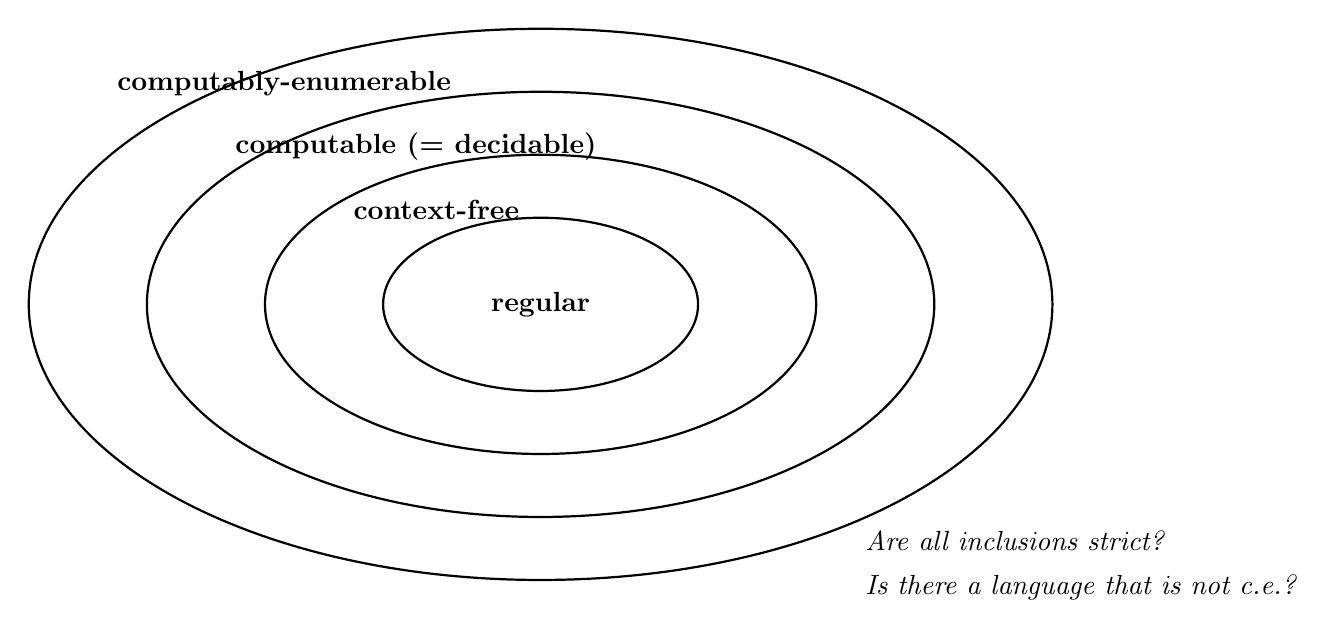
\begin{tikzpicture}
\draw[thick] (0,0) ellipse (6.5cm and 3.5cm);
\node[anchor=west] at (-5.5,2.8) {\textbf{computably-enumerable}};
\draw[thick] (0,0) ellipse (5cm and 2.7cm);
\node[anchor=west] at (-4,2.0) {\textbf{computable (= decidable)}};
\draw[thick] (0,0) ellipse (3.5cm and 1.9cm);
\node[anchor=west] at (-2.5,1.2) {\textbf{context-free}};
\draw[thick] (0,0) ellipse (2cm and 1.1cm);
\node at (0,0) {\textbf{regular}};
\node[anchor=west] at (4,-3) {\textit{Are all inclusions strict?}};
\node[anchor=west] at (4,-3.6) {\textit{Is there a language that is not c.e.?}};
\end{tikzpicture}
\end{center}

\begin{itemize}[nosep]
\item \textbf{Regular $\subset$ context-free}: You know this from Semester 1. $\{0^n 1^n\}$ is context-free but not regular.
\item \textbf{Context-free $\subset$ computable}: There exist computable languages that are not context-free. (E.g., $\{0^n 1^n 2^n\}$.)
\item \textbf{Computable $\subset$ c.e.}: There exist c.e.\ languages that are not computable. (The Halting Problem --- Lecture 2.)
\item \textbf{C.e.\ $\subset$ all languages}: There exist languages that are not even c.e.! (Lecture 3.)
\end{itemize}

\textbf{The big questions} the slides pose (answered in Lectures 2--3):
\begin{enumerate}[nosep]
\item Are all these inclusions \textbf{strict}? Yes.
\item Is there a language that is \textbf{not even c.e.}? Yes --- and we'll prove it using \textbf{diagonalization}.
\end{enumerate}


%═══════════════════════════════════════════════════════════════════════════════
\subsection{A Note on Terminology (slide 32)}

\begin{center}
\renewcommand{\arraystretch}{1.4}
\begin{tabular}{lll}
\toprule
\textbf{This course says} & \textbf{Other books say} & \textbf{Same concept} \\
\midrule
Halting TM & Decider & A TM that always stops \\
Computable & Decidable & $\exists$ halting TM with $L(M) = L$ \\
Computably-enumerable & Semi-decidable / r.e. & $\exists$ TM (any) with $L(M) = L$ \\
\bottomrule
\end{tabular}
\end{center}

If you read Sipser's book or other sources, they use the right column. Same concepts, different names. Don't get confused.


%═══════════════════════════════════════════════════════════════════════════════
\subsection{The Conclusion Slide (slide 33)}

This is the most important slide of the lecture. It summarizes everything:

\begin{conceptbox}{Lecture 1 --- The Three Things We Learned}

\textbf{1. Problems = Formal Languages}

Every decision problem is equivalent to a language $L \subseteq \Sigma^*$.

\textbf{2. DTMs as an abstract model of computation}

A DTM is a 7-tuple that precisely defines ``algorithm.'' This lets us reason mathematically about what can and can't be computed.

\textbf{3. Computable vs.\ Computably-Enumerable --- THE distinction:}

\renewcommand{\arraystretch}{1.4}
\begin{center}
\begin{tabular}{p{3.5cm}p{5cm}p{5cm}}
\toprule
& \textbf{Computably-enumerable} & \textbf{Computable} \\
\midrule
Machine & $\exists$ DTM $M$ with $L(M) = L$ & $\exists$ \textbf{halting} DTM $M$ with $L(M) = L$ \\
$w \in L$ & $M$ accepts $w$ & $M$ accepts $w$ \\
$w \notin L$ & $M$ rejects $w$ \textbf{or loops} & $M$ rejects $w$ \\
\bottomrule
\end{tabular}
\end{center}

\textbf{And:} the slide says ``too many slides'' --- this was a dense lecture.
\end{conceptbox}


%═══════════════════════════════════════════════════════════════════════════════
\newpage
\section{How to Build a Turing Machine}
%═══════════════════════════════════════════════════════════════════════════════

This section doesn't correspond to a specific slide, but it's what you need to do Exercises 4 and 5. Think of it as the ``applied skills'' section.

\subsection{The General Strategy}

\begin{notebox}{Step-by-Step Guide to Constructing a DTM}
\begin{enumerate}
\item \textbf{Understand the language.} What strings are in $L$? What strings are not? Write down 3--4 examples of each.

\item \textbf{Describe the algorithm in English first.} How would YOU decide membership if you had a tape and a pencil? What would you scan for? What would you compare?

\item \textbf{Identify the phases.} Most TM algorithms have phases: ``scan right to find X'', ``go back to check Y'', ``erase and repeat.'' Each phase becomes a state (or group of states).

\item \textbf{Use states to encode memory.} A TM's only ``memory'' beyond the tape is its state. If you need to remember that you saw a 1, create a state $q_{\text{saw1}}$. If you need to carry a symbol across the tape, encode it in the state name: $q_\ell^0$ (carrying 0) vs.\ $q_\ell^1$ (carrying 1).

\item \textbf{Write the transition table.} For each (state, symbol) pair, decide: what state next? what symbol to write? which direction to move?

\item \textbf{Test on examples.} Trace through your TM on at least: one accepting input, one rejecting input, and the empty string $\varepsilon$.

\item \textbf{Check: does it halt on all inputs?} If the exercise asks for a halting DTM, verify there's no input that causes looping.
\end{enumerate}
\end{notebox}

\subsection{The Key Technique: Using States as Memory}

\begin{conceptbox}{States = Memory}
A Turing machine has no variables, no registers, no stack. The ONLY way to ``remember'' something is:
\begin{enumerate}[nosep]
\item \textbf{Write it on the tape} (you can always go back and read it)
\item \textbf{Encode it in the state} (change to a different state depending on what you saw)
\end{enumerate}

\textbf{Example:} To check if the first letter equals the last letter:
\begin{itemize}[nosep]
\item Read the first letter. If it's 0, go to state $q_{\text{first0}}$. If it's 1, go to state $q_{\text{first1}}$.
\item Scan right to the end of the input.
\item Read the last letter.
\item In state $q_{\text{first0}}$: accept if last letter is 0, reject if 1.
\item In state $q_{\text{first1}}$: accept if last letter is 1, reject if 0.
\end{itemize}

The ``memory'' of what the first letter was is stored in whether we're in state $q_{\text{first0}}$ or $q_{\text{first1}}$.
\end{conceptbox}


%═══════════════════════════════════════════════════════════════════════════════
\newpage
\section{Summary --- Key Concepts Quick Reference}
%═══════════════════════════════════════════════════════════════════════════════

\begin{center}
\renewcommand{\arraystretch}{1.5}
\begin{tabular}{lp{11cm}}
\toprule
\textbf{Concept} & \textbf{One-liner} \\
\midrule
Decision problem & A yes/no question about inputs. Formalized as a language $L \subseteq \Sigma^*$. \\
DTM & 7-tuple $(Q, \Sigma, \Gamma, s, t, r, \delta)$: states, input alphabet, tape alphabet, start, accept, reject, transition function. \\
$\Sigma$ vs $\Gamma$ & $\Sigma$ = input symbols. $\Gamma \supseteq \Sigma$ = tape symbols (includes blank $\sqcup$). $\sqcup \in \Gamma \setminus \Sigma$. \\
$\delta$ domain & $\delta\colon (Q \setminus \{t,r\}) \times \Gamma \to Q \times \Gamma \times \{-1,+1\}$. No rules for $t$ or $r$. \\
Configuration & Snapshot $[q, \tau, \ell]$: current state, tape contents, head position. \\
Initial config & $[s, w\sqcup\ldots, 1]$ for input $w$. \\
Successor & From $[q,\tau,\ell]$: if $\delta(q,\tau(\ell)) = (p,a,d)$, then $[p,\tau',\max\{\ell+d,1\}]$. \\
$\alpha \vdash_M \beta$ & One computation step. \\
$\alpha \vdash_M^n \beta$ & Exactly $n$ steps. \\
$\alpha \vdash_M^* \beta$ & Some number of steps ($\geq 0$). \\
Accept & $\exists$ accepting config reachable from initial config. \\
Reject & $\exists$ rejecting config reachable from initial config. \\
Loop & Neither accept nor reject. Runs forever. \\
$L(M)$ & $\{w \in \Sigma^* \mid M$ accepts $w\}$. \\
Halting DTM & Halts (accepts or rejects) on \textbf{every} input. Never loops. \\
Computable & $\exists$ halting DTM $M$ with $L = L(M)$. No input causes looping. \\
C.e. & $\exists$ DTM $M$ with $L = L(M)$. May loop on inputs $\notin L$. \\
\bottomrule
\end{tabular}
\end{center}

\subsection{Common Pitfalls}

\begin{conceptbox}{Things That Will Trip You Up}
\begin{enumerate}
\item \textbf{$\Sigma$ vs $\Gamma$}: The blank $\sqcup$ is in $\Gamma$ but NOT in $\Sigma$. A DTM \textit{can} write $\sqcup$ on the tape (this is how you ``erase'' a symbol). But $\sqcup$ never appears in the original input.

\item \textbf{Can $\Gamma = \Sigma$?} No! Because $\sqcup \in \Gamma \setminus \Sigma$, we need $\Gamma \supsetneq \Sigma$ (strict superset --- at least the blank is extra).

\item \textbf{$t$ and $r$ are not in $\delta$'s domain}: $\delta$ is defined on $(Q \setminus \{t,r\}) \times \Gamma$. There's no transition from $t$ or $r$. Reaching $t$ or $r$ = stop.

\item \textbf{The head can't go left of position 1}: $\max\{\ell + d, 1\}$ ensures this. If you're at position 1 and move left, you stay at 1.

\item \textbf{Can the head stay on the same cell?} No! The direction $d \in \{-1, +1\}$ --- there's no 0 option. The head MUST move left or right every step.

\item \textbf{Given state $q \neq t,r$ reading symbol $a$, how many possible next configurations?} Exactly \textbf{one}. $\delta$ is a function (deterministic), so $\delta(q,a)$ has exactly one value.

\item \textbf{If $L$ is computable, is it c.e.?} YES. Every halting DTM is a DTM. So $L$ computable $\Rightarrow$ $L$ c.e.

\item \textbf{Empty input $\varepsilon$}: Don't forget this case. On empty input, the tape is all blanks, and the head reads $\sqcup$ immediately in state $s$.

\item \textbf{``Not in $L(M)$'' $\neq$ ``$M$ rejects''}: $w \notin L(M)$ if $M$ rejects OR loops on $w$. Only for halting DTMs can you equate ``not in $L(M)$'' with ``$M$ rejects.''
\end{enumerate}
\end{conceptbox}

\subsection{What to Handwrite After Reading This}

\begin{itemize}[nosep]
\item The 7-tuple definition of a DTM with all components explained
\item The configuration $[q, \tau, \ell]$ and successor formula
\item The computable vs.\ c.e.\ comparison table
\item The $\vdash_M$, $\vdash_M^n$, $\vdash_M^*$ definitions
\item A small worked TM example with full trace
\item The hierarchy: regular $\subset$ context-free $\subset$ computable $\subset$ c.e.
\end{itemize}

\subsection{Reading (slide 34)}
\begin{itemize}[nosep]
\item ``Computability and Complexity'' by Hubie Chen: Introduction (pp.\ xiii--xvii), Section 2.1 (pp.\ 71--85)
\item Skim Section 1 (pp.\ 1--21) for notation and DFA refresher
\item Turing's 1936 paper: \texttt{https://www.cs.virginia.edu/\textasciitilde robins/Turing\_Paper\_1936.pdf}
\end{itemize}

\end{document}
